\chapter{Systemarchitektur und Implementierung} \label{implementierung}
% Der \gls{accesspoint} sendet die \gls{bssid} und die \gls{ssid}, damit Geräte, wie eine \gls{vm}, sich verbinden können. Algorithmen wie \gls{knn} und \gls{svm} können in einer \gls{api} implementiert werden, um die Datenverarbeitung zu optimieren.

Die implementierte Software lässt sich in vier Komponenten unterteilen: Die Android App \textit{BVG Detection}, welche bereits in einer vorherigen Arbeit entwickelt wurde\myfootcite{winter2017indoor}{S. 11 ff.}, einem Server der eine API bereitstellt, welche die in der Offline-Phase gesammelten Daten speichern kann und für WiFi-Fingerprints von unbekannten Räumen eine Vorhersage treffen kann, einer Datenbank zur Verwaltung der Fingerprints und dem Quellcode der Microcontroller.

\section{Datenbankstruktur} \label{datenbank}

Für die Speicherung der gesammelten WiFi-Fingerprints während der Offline-Phase wurde eine Datenbankstruktur entwickelt, welche auf einer \textit{MariaDB}-Instanz auf dem Server und in einer \textit{SQLite}-Datenbank innerhalb der App \textit{BVG Detection} implementiert wurde. Die Datenbank besteht aus den vier Tabellen \texttt{rooms}, \texttt{measurements}, \texttt{routers} und \texttt{measurement\_router}.

\subsection{Tabelle \texttt{rooms}}

In der Tabelle \texttt{rooms} werden die Informationen der Räume, in denen die Messungen durchgeführt wurden, gespeichert. Dazu gehören eine eindeutige Raum-ID, der Name des Raumes, eine Beschreibung,  Koordinaten und der Pfad zu einer Bilddatei. Die Beschreibung, die Koordinaten und der Pfad der Bilddatei sind dabei nur für die \textit{BVG Detection}-App relevant.

\begin{table}[h]
    \centering
    \begin{tabularx}{\textwidth}{|l|l|X|}
        \hline
        \textbf{Spalte} & \textbf{Datentyp} & \textbf{Beschreibung} \\ \hline
        room\_id & INT & Primärschlüssel der Tabelle \\ \hline
        room\_name & VARCHAR(255) & Eindeutiger Name des Raumes \\ \hline
        description & VARCHAR(255) & Beschreibung des Raumes \\ \hline
        coordinates & VARCHAR(255) & Geografische Koordinaten des Raumes \\ \hline
        picture\_path & VARCHAR(255) & Pfad zu einer Bilddatei des Raumes \\ \hline
    \end{tabularx}
    \caption{Struktur der Tabelle \texttt{rooms}.}
    \label{tab:rooms}
\end{table}

\subsection{Tabelle \texttt{measurements}}

Die Tabelle \texttt{measurements} dient der Erfassung aller Messungen. Jede Messung wird durch eine eindeutige Kombination aus Geräte-ID und Zeitstempel identifiziert, um doppelte Einträge zu vermeiden. Das ist wichtig, da in einer Datenbank auch die Messungen mehrerer Geräte vorhanden sein können und diese unterschieden werden müssen. Zudem wird die Raum-ID gespeichert, die auf die Tabelle \texttt{rooms} verweist, wodurch die Messung einem Raum zugeordnet werden kann.

\begin{table}[h]
    \centering
    \begin{tabularx}{\textwidth}{|l|l|X|}
        \hline
        \textbf{Spalte} & \textbf{Datentyp} & \textbf{Beschreibung} \\ \hline
        measurement\_id & INT & Primärschlüssel der Tabelle \\ \hline
        timestamp & TIMESTAMP & Zeitpunkt der Messung \\ \hline
        device\_id & VARCHAR(255) & ID des Gerätes, das die Messung durchgeführt hat \\ \hline
        room\_id & INT & Verweis auf den Raum, in dem die Messung stattfand \\ \hline
    \end{tabularx}
    \caption{Struktur der Tabelle \texttt{measurements}.}
    \label{tab:measurements}
\end{table}

\subsection{Tabelle \texttt{routers}}

In der Tabelle \texttt{routers} werden die Informationen der erfassten Access Points gespeichert. Die Einträge der Spalte \textit{BSSID} werden dazu verwendet, um zu überprüfen, ob ein Access Point bereits in der Tabelle gespeichert ist, da die \textit{BSSID} jeden Access Point eindeutig kennzeichnet.

\begin{table}[h]
    \centering
    \begin{tabularx}{\textwidth}{|l|l|X|}
        \hline
        \textbf{Spalte} & \textbf{Datentyp} & \textbf{Beschreibung} \\ \hline
        router\_id & INT  & Primärschlüssel der Tabelle \\ \hline
        ssid & VARCHAR(255) & Name des WiFi-Netzwerks (SSID) \\ \hline
        bssid & VARCHAR(255) & MAC-Adresse des Routers (BSSID) \\ \hline
    \end{tabularx}
    \caption{Struktur der Tabelle \texttt{routers}.}
    \label{tab:routers}
\end{table}

\subsection{Tabelle \texttt{measurement\_router}}


Die Tabelle \textit{measurement\_router} speichert die empfangenen Signalstärken der Access Points aller Messungen und verknüpft diese über den Eintrag \textit{measurement\_id} mit den Einträgen aus der Tabelle \textit{measurements}. 

\begin{table}[h]
    \centering
    \begin{tabularx}{\textwidth}{|l|l|X|}
        \hline
        \textbf{Spalte} & \textbf{Datentyp} & \textbf{Beschreibung} \\ \hline
        measurement\_id & INT & Verweis auf eine Messung \\ \hline
        router\_id & INT & Verweis auf einen Router \\ \hline
        signal\_strength & INT & Empfangene Signalstärke bei der Messung \\ \hline
    \end{tabularx}
    \caption{Struktur der Tabelle \texttt{measurement\_router}.}
    \label{tab:measurement_router}
\end{table}

\section{Implementierung des Servers} \label{api}

% Quelle: https://dev.to/ken_mwaura1/getting-started-monitoring-a-fastapi-app-with-grafana-and-prometheus-a-step-by-step-guide-3fbn

Der Server läuft auf einer virtuellen Maschine der HTW Berlin unter der Linux Distribution \textit{Debain}, ist mit 2 CPU-Kernen, 3 GB RAM und einem Speicherplatz von 16 GB konfiguriert und ist über die IP-Adresse \texttt{141.45.212.246} aus dem Netzwerk der HTW erreichbar. Auf diesem Server sind vier zentrale Anwendungen in separaten Docker-Containern implementiert: eine \textit{FastAPI}-Anwendung, \textit{Prometheus}, \textit{Grafana} und \textit{MariaDB}. Diese Anwendungen können mithilfe von \textit{Docker Compose} über den Befehl \texttt{sudo docker-compose build} installiert werden und über \texttt{sudo docker-compose up -d} und \texttt{sudo docker-compose down} gestartet bzw. beendet werden. Das bietet den Vorteil, dass alle Anwendungen ohne großen Aufwand installiert werden können und die Abhängigkeiten der Anwendungen korrekt konfiguriert sind. Die Implementierung des Servers basiert auf der Anleitung von \textit{Zoo Codes}.\mycitefoot{devGettingStarted}

\subsection{FastAPI} \label{section-fastapi}

% Verwendet: sqlalchemy

% Quelle Vorteile FastAPI https://www.netguru.com/blog/python-flask-versus-fastapi
Die API zur Verwaltung von WiFi-Fingerprints und zur Vorhersage von Räumen basierend auf WiFi-Fingerprints von nicht bekannten Räumen wurde mithilfe des Python-Frameworks \textit{FastAPI} implementiert. \textit{FastAPI} bietet den Vorteil, dass automatisch eine interaktive API-Dokumentation (aufrufbar unter \texttt{http://141.45.212.246:8000/docs}) bereitgestellt wird (siehe Abbildung \ref{fig:fast_api_screenshot}), die es ermöglicht, die Endpunkte der API zu testen.

\begin{figure}[h]
    \centering
    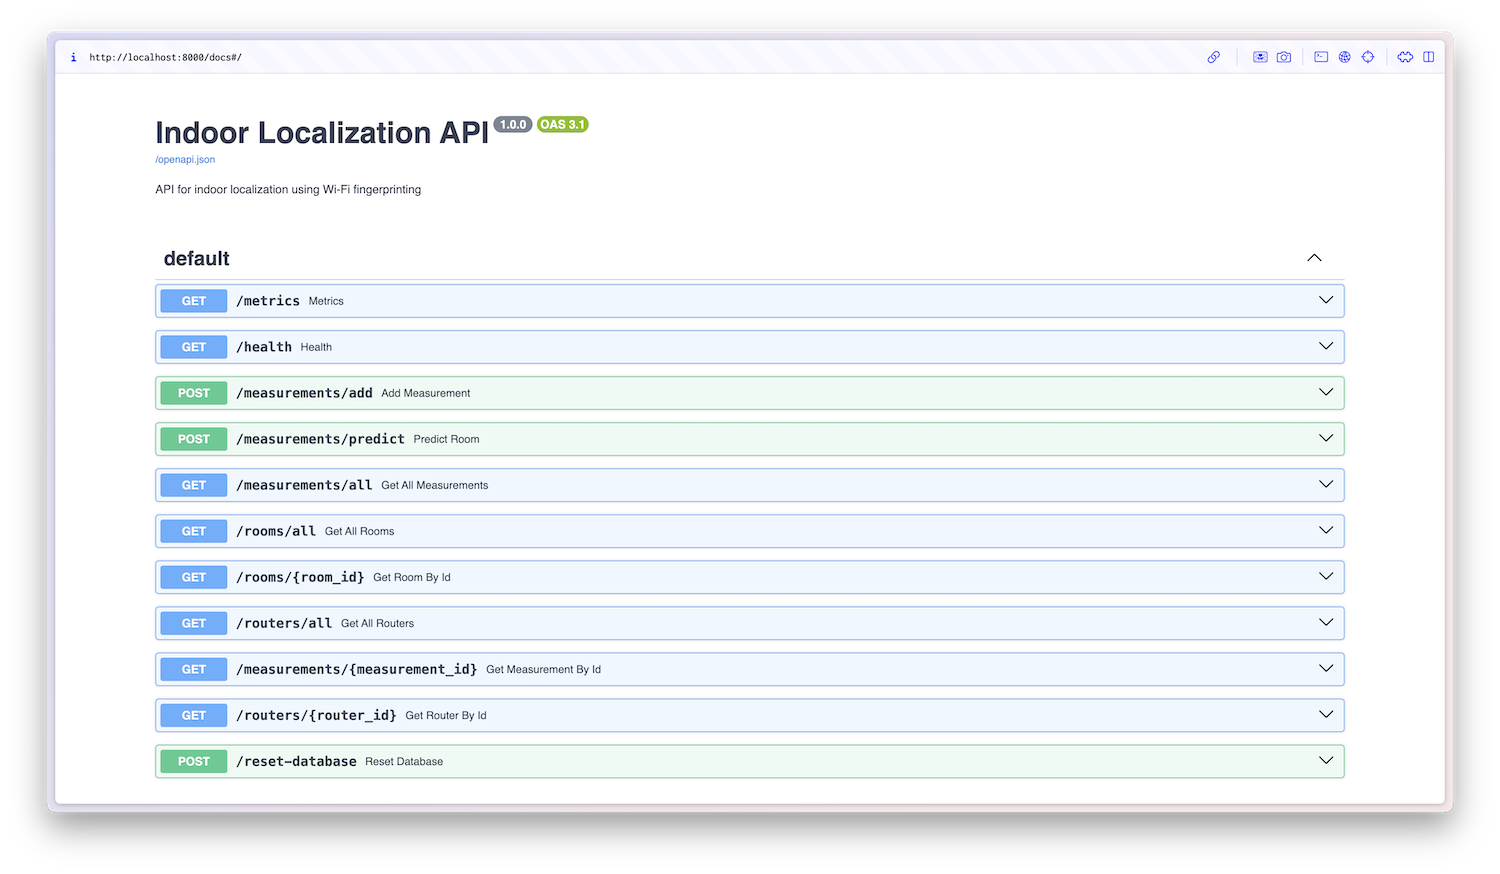
\includegraphics[width=0.8\textwidth]{images/screenshots/api_docs.png}
    \caption{FastAPI Dokumentation}
    \label{fig:fast_api_screenshot}
\end{figure}

Die API stellt verschiedene Routen zur Verfügung, welche in Tabelle \ref{tab:api_routes} aufgelistet sind.

\begin{table}[h]
    \centering
    \begin{tabularx}{\textwidth}{|l|l|X|}
    \hline
    \textbf{Route} & \textbf{Methode} & \textbf{Beschreibung} \\ \hline
    \texttt{/health} & \texttt{GET} & Prüft den Status der API. \\ \hline
    \texttt{/measurements/add} & \texttt{POST} & Fügt eine neue Messung hinzu. \\ \hline
    \texttt{/measurements/predict} & \texttt{POST} & Sagt den Raum basierend auf Wi-Fi-Daten voraus. \\ \hline
    \texttt{/measurements/all} & \texttt{GET} & Ruft alle gespeicherten Messungen ab. \\ \hline
    \texttt{/measurements/\{measurement\_id\}} & \texttt{GET} & Ruft eine spezifische Messung nach ID ab. \\ \hline
    \texttt{/rooms/all} & \texttt{GET} & Ruft alle gespeicherten Räume ab. \\ \hline
    \texttt{/rooms/\{room\_id\}} & \texttt{GET} & Ruft einen spezifischen Raum nach ID ab. \\ \hline
    \texttt{/routers/all} & \texttt{GET} & Ruft alle gespeicherten Router ab. \\ \hline
    \texttt{/routers/\{router\_id\}} & \texttt{GET} & Ruft einen spezifischen Router nach ID ab. \\ \hline
    \texttt{/reset-database} & \texttt{POST} & Setzt die Datenbank zurück. \\ \hline
    \end{tabularx}
    \caption{Übersicht der Endpunkte der \textit{FastAPI}-Anwendung.}
    \label{tab:api_routes}
\end{table}

\subsection*{Route: \texttt{/measurements/add}}

Zum Hinzufügen eines neuen WiFi-Fingerprints, der während der Offline-Phase gesammelt wurde, kann die Route \texttt{/measurements/add} verwendet werden. Dabei wird im ersten Schritt überprüft, ob es bereits einen Eintrag in der Tabelle \texttt{measurements} gibt, bei dem die Einträge \texttt{device\_id} und \texttt{timestamp} mit den übergebenen Werten übereinstimmen. Falls ein solcher Eintrag bereits existiert, wird die Messung nicht hinzugefügt. Dadurch kann sichergestellt werden, dass keine doppelten Einträge in der Datenbank vorhanden sind. Sollte die Messung noch nicht in der Datenbank vorhanden sein, wird für diese Messung ein neuer Eintrag in der Tabelle \texttt{measurements} hinzugefügt und für jeden empfangenen Router ein Eintrag in der Tabelle \texttt{measurement\_router} erstellt.

In dem Code Beispiel \ref{lst:add_request} ist eine Beispielanfrage an die Route \texttt{/measurements/add} dargestellt, bei der ein neuer WiFi-Fingerprint für den Raum \texttt{WH\_C\_625} hinzugefügt werden soll.

\begin{lstlisting}[caption={Beispiel für eine Anfrage an \texttt{/measurements/predict}}, label={lst:add_request}]
{
    "room_name": WH_C_625,
    "device_id": google_pixel_8,
    "timestamp": 1721479799,
    "routers": [
        {
            "ssid": "eduroam",
            "bssid": "dc:b8:08:c9:73:02",
            "signal_strength": -73
        }
    ]
}
\end{lstlisting}

\subsection*{Route: \texttt{/measurements/predict}}

Die \texttt{POST} Route \texttt{/measurements/predict} wird verwendet um für einen WiFi-Fingerprint eine Raumvorhersage zu treffen. Dafür wurden die in Kapitel \ref{algorithmen} beschriebenen Algorithmen \gls{knn}, \gls{svm} und Random Forest mit den dazugehörigen Parametern implementiert. Für die Implementierung der Algorithmen wurde die Python Bibliothek \texttt{scikit-learn} verwendet.

Der Endpunkt erwartet unter dem Parameter \texttt{routers} eine Liste von Router Objekten, welche jeweils die Einträge \texttt{ssid}, \texttt{bssid} und \texttt{signal\_strength} beinhalten. Zusätzlich kann über den optionalen Parameter \texttt{algorithm} der Algorithmus zur Vorhersage festgelegt werden (die möglichen Werte hierbei sind \texttt{knn\_euclidean}, \texttt{knn\_sorensen}, \texttt{random\_forest}, \texttt{svm\_rbf} und \texttt{svm\_linear}). Die Algorithmus spezifischen Parameter können über die Parameter \texttt{k\_value}, \texttt{weights}, \texttt{n\_estimators}, \texttt{c\_value}, \texttt{gamma\_value}, \texttt{max\_depth} und \texttt{max\_features} gesetzt werden und entsprechen den Parametern der \texttt{scikit-learn} Bibliothek. Über den Parameter \texttt{ignore\allowbreak\_\allowbreak measurements} können \textit{IDs} von Messungen angegeben werden, die bei der Vorhersage ignoriert werden sollen.

Für die Verwendung der in Kapitel \ref{strategien} untersuchten Datenaufbereitungsmethoden können die Parameter \texttt{use\allowbreak\_remove\allowbreak\_unreceived\allowbreak\_bssids}, \texttt{handle\allowbreak\_missing\allowbreak\_values\allowbreak\_strategy}, \texttt{router\allowbreak\_selection}, \texttt{router\allowbreak\_presence\allowbreak\_threshold}, \texttt{value\allowbreak\_scaling\allowbreak\_strategy} und \texttt{router\allowbreak\_rssi\allowbreak\_thres\-hold} gesetzt werden.

In dem Code Beispiel \ref{lst:predict_request} ist eine Beispielanfrage an die Route \texttt{/measurements/predict} dargestellt, bei der für einen WiFi-Fingerprint bestehend aus zwei Access Points eine Raumvorhersage getroffen werden soll unter Verwendung des \gls{knn}-Algorithmus mit dem Wert 5 für k und ohne Gewichtungsfunktion (\texttt{weights = uniform}).

\begin{lstlisting}[caption={Beispiel für eine Anfrage an \texttt{/measurements/predict}}, label={lst:predict_request}]
{
    "routers": [
        {
            "ssid": "eduroam",
            "bssid": "dc:b8:08:c9:54:a1",
            "signal_strength": -88
        },
        {
            "ssid": "Gast@HTW",
            "bssid": "dc:b8:08:c9:54:a2",
            "signal_strength": -85
        }
    ],
    "algorithm": "knn_euclidean",
    "k_value": 5,
    "weights": "uniform"
}
\end{lstlisting}

Als Antwort liefert die API ein \textit{JSON}-Objekt, das den vorhergesagten Raum zurückgibt.

\begin{lstlisting}[caption={Beispiel einer API-Antwort von \texttt{/measurements/predict}}]
{
  "room_name": "WH_C_625",
}
\end{lstlisting}

\subsection{Grafana und Prometheus}

Neben der Datenbank und der FastAPI-Anwendung wurden auch die Monitoring-Tools \texttt{Pro\discretionary{-}{}{}metheus} und \texttt{Grafana} auf dem Server installiert, um die Leistung der Anwendungen zu überwachen und die Daten in Echtzeit zu visualisieren. Dabei dient Prometheus zur Speicherung der Metriken von der \textit{FastAPI} und \textit{Grafana} zur Visualisierung. Für die Überwachung der \textit{FastAPI} wurde ein Dashboard implementiert, welches die CPU- und RAM-Auslastung, die Anfragen pro Minute nach \textit{HTTP}-Statuscode und die durchschnittliche Antwortzeit für jeden Endpunkt anzeigt (siehe Abbildung \ref{fig:grafana_fast_api_screenshot}).  

\begin{figure}[h]
    \centering
    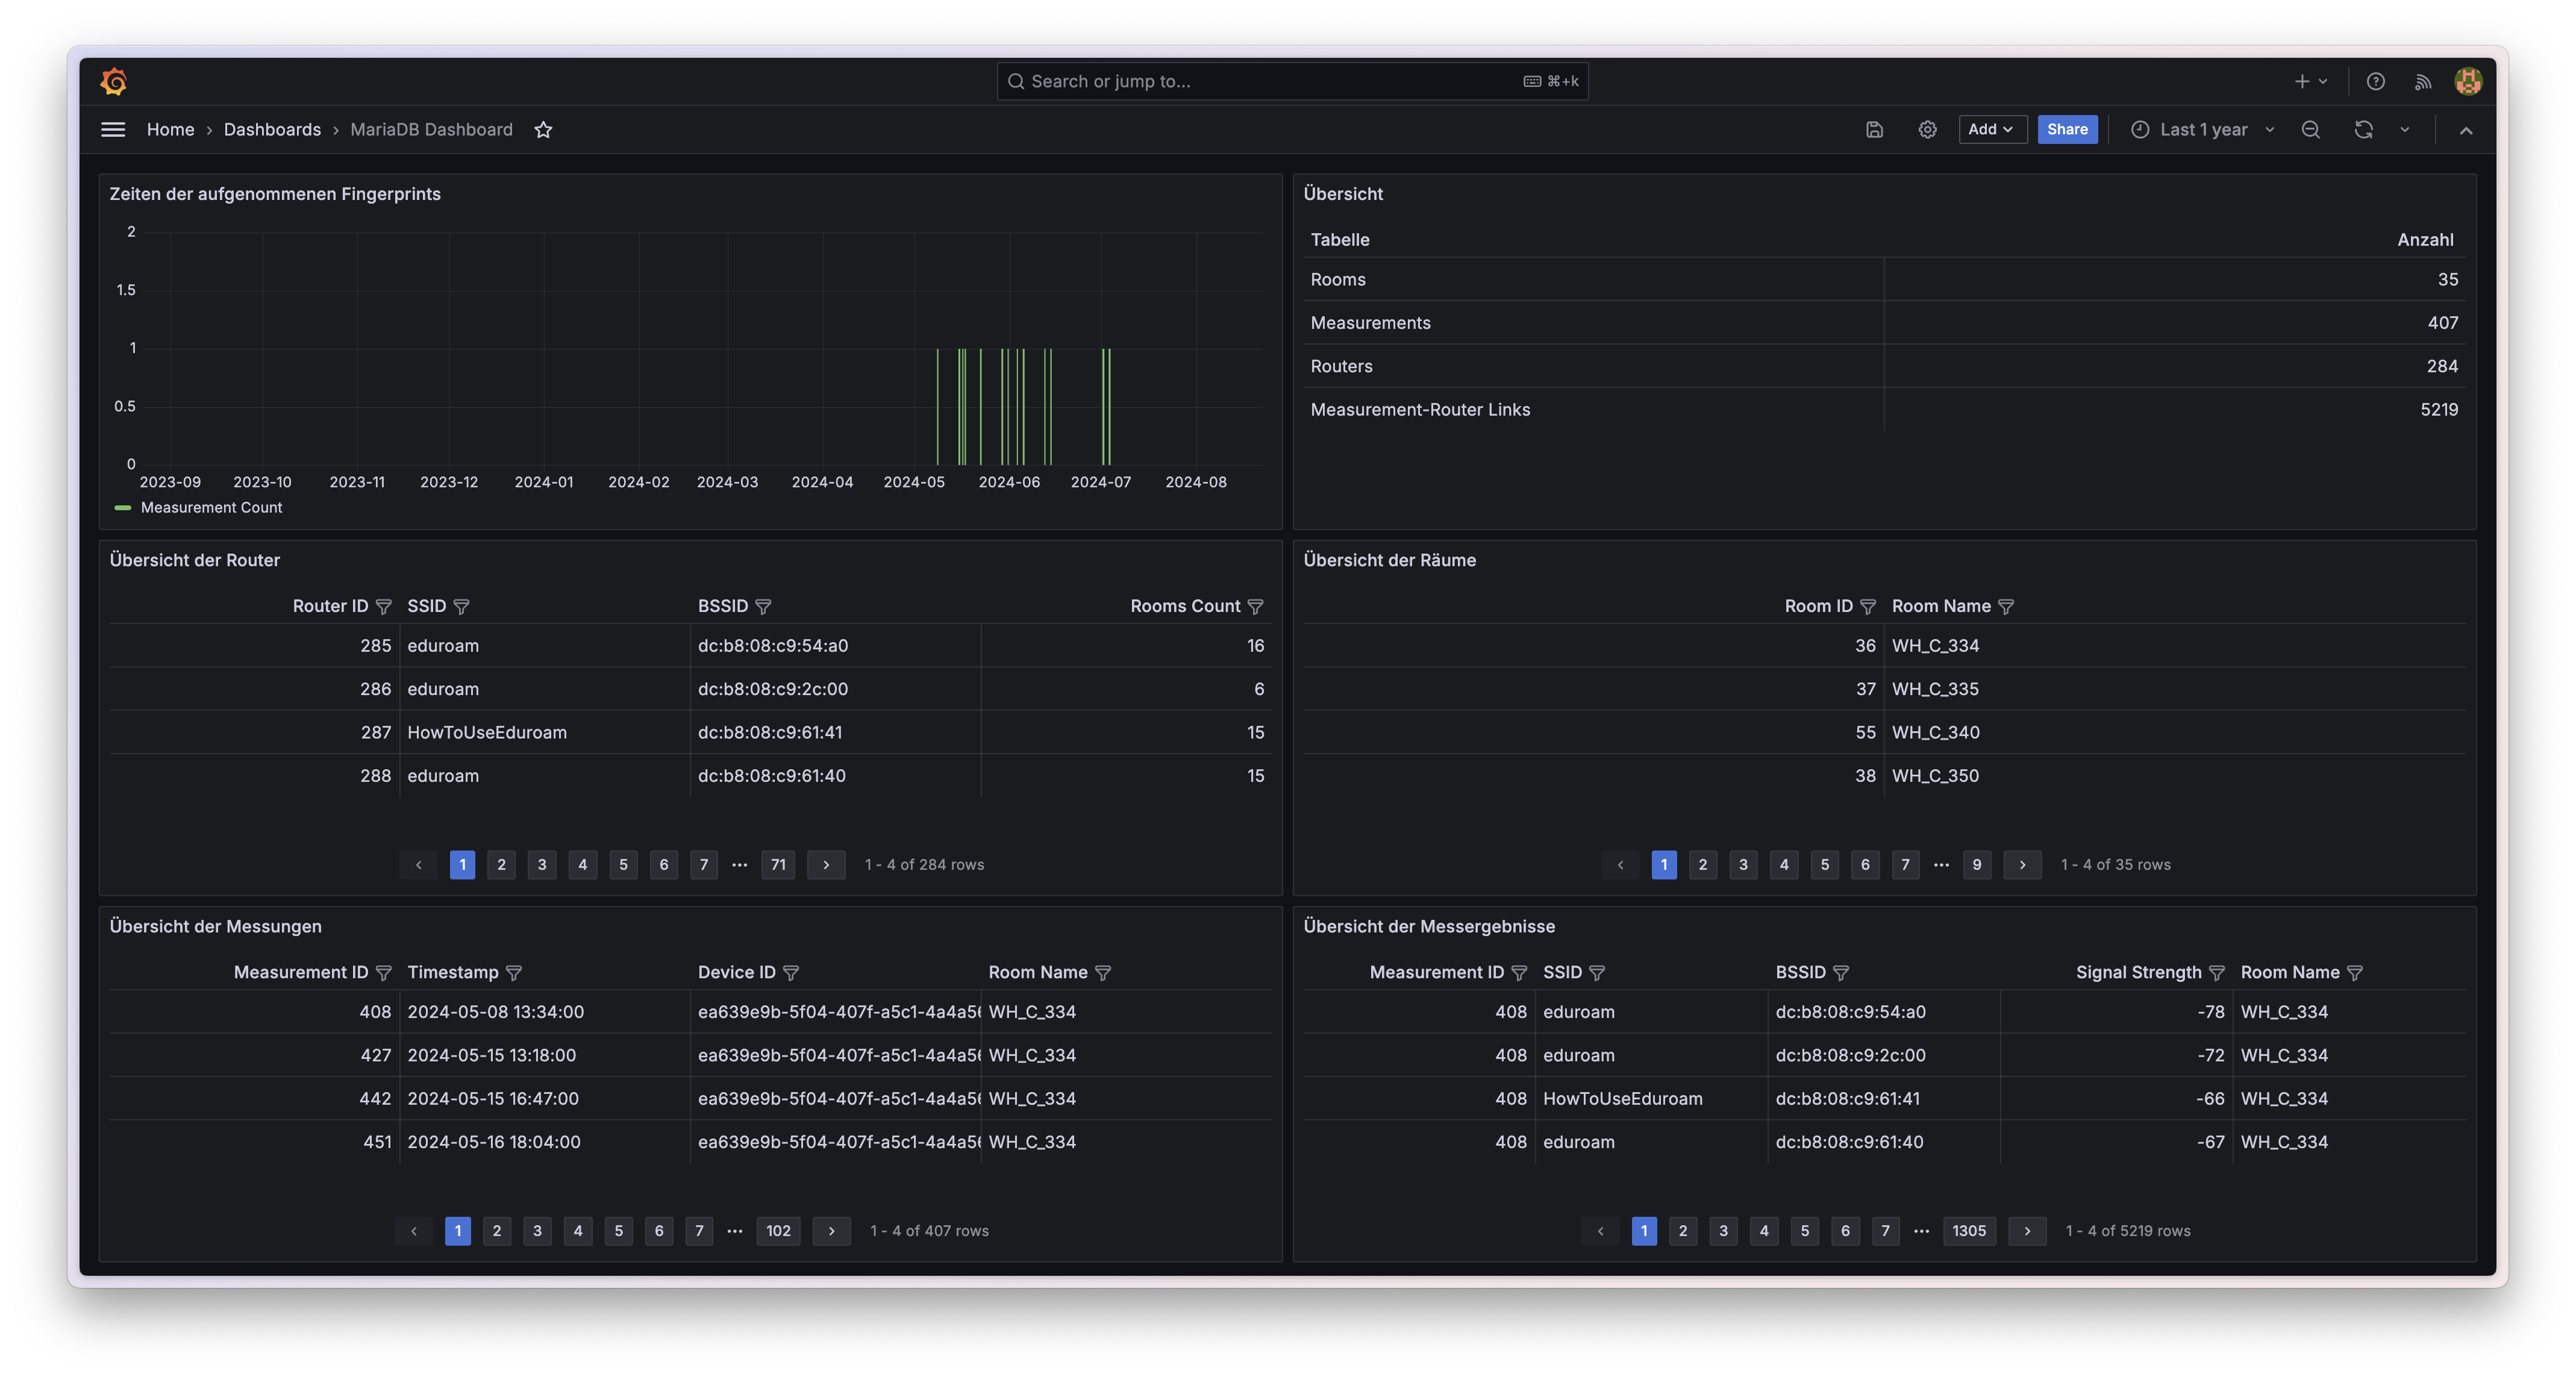
\includegraphics[width=0.8\textwidth]{images/grafana_fast_api_screenshot.png}
    \caption{Grafana Dashboard der \textit{FastAPI}}
    \label{fig:grafana_fast_api_screenshot}
\end{figure}

Für die Visualisierung der \textit{MariaDB} wurde ebenfalls ein \textit{Grafana}-Dashboard erstellt, welches eine Übersicht der Datenbank, die Inhalte der Tabellen und die Zeitpunkte darstellt, an denen die Messungen durchgeführt wurden (siehe Abbildung \ref{fig:grafana_maria_db_screenshot}). Die Dashboards können aus dem Netz der HTW über Adresse \texttt{http://141.45.212.246:3000} aufgerufen werden.

\begin{figure}[h]
    \centering
    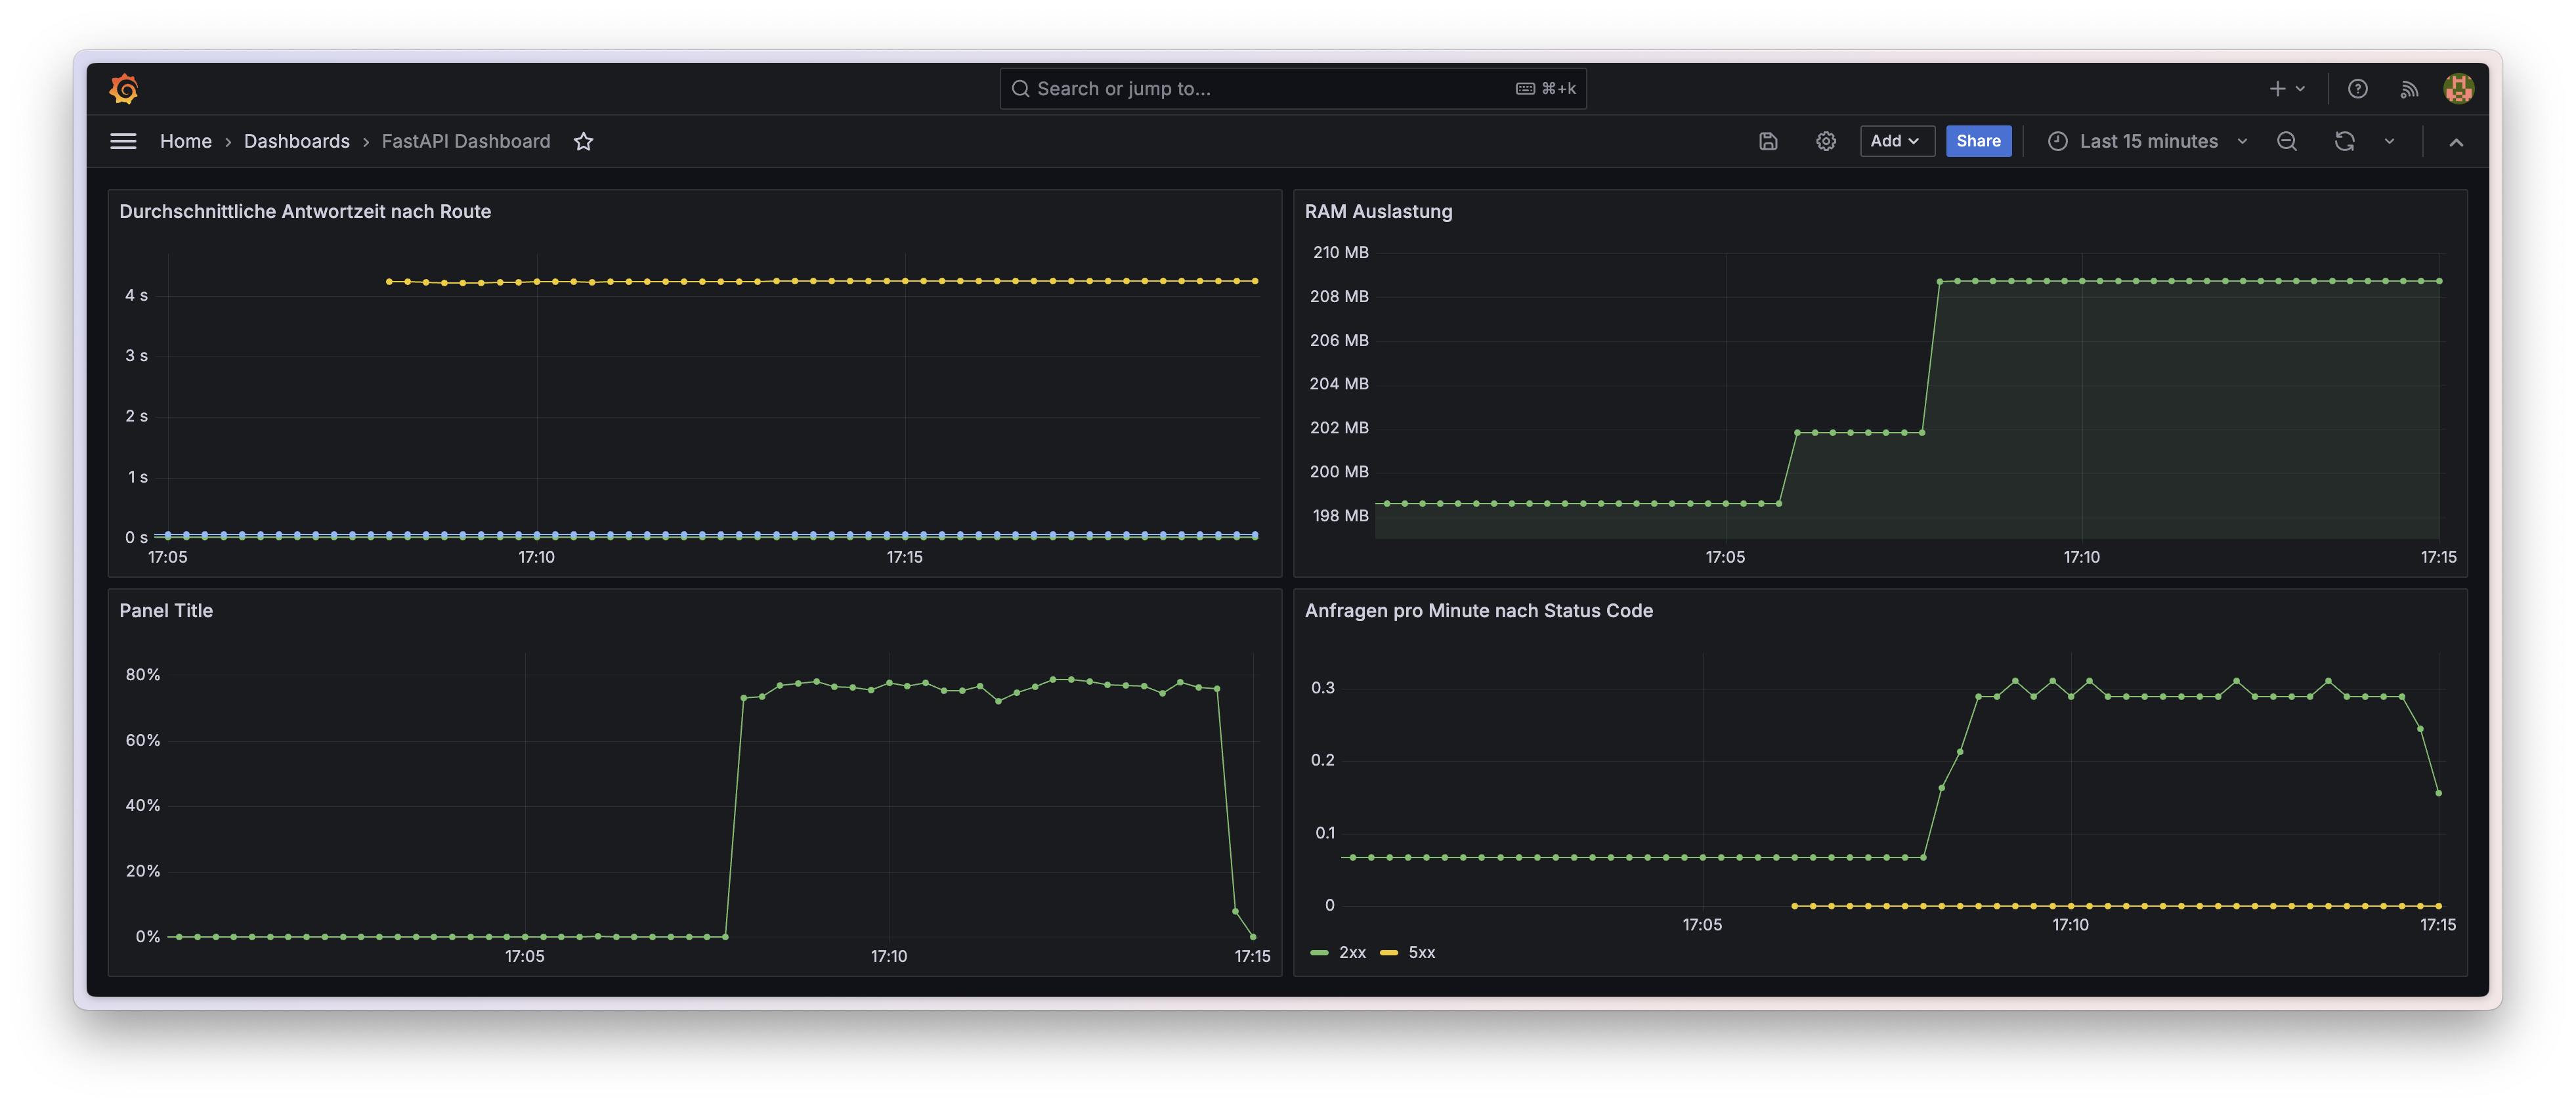
\includegraphics[width=0.8\textwidth]{images/grafana_maria_db_screenshot.png}
    \caption{Grafana Dashboard der \textit{MariaDB}}
    \label{fig:grafana_maria_db_screenshot}
\end{figure}

\section{Implementierung der \textit{BVG Detection} App}

Die Android App \textit{BVG Detection} (\url{https://github.com/OpenHistoricalDataMap/BVGDetection}) kann unteranderem dazu verwendet werden WiFi-Fingerprints von Orten zu speichern und die eigene Position anhand der bekannten WiFi-Fingerprints zu bestimmen. 

Die bisherige Implementierung wurde um die Funktionalität erweitert mehr als einen Fingerprint pro Raum aufzunehmen und die in der Offline Phase gemessenen Fingerprints mit anderen Geräten und der API auszutauschen. Zudem wurden die untersuchten Algortihmen aus dieser Arbeit für die Raumvorhersage implementiert.

\subsection{Wiederinbetriebnahme der App}

In der bisherigen Implementierung konnte die App zum Zeitpunkt dieser Arbeit nicht mehr kompiliert werden. Dies lag daran, dass das verwendete Build-Tool \textit{Gradle} veraltet war und in der aktuellen Version von \textit{Android Studio (Koala | 2024.1.1)} nicht mehr unterstützt wurde. Damit die App wieder kompiliert werden konnte, wurde \textit{Gradle} von der Version \texttt{2.3.3} auf die Version \texttt{8.3.2} aktualisiert.\mycitefoot{androidAndroidGradle} % https://developer.android.com/build/releases/gradle-plugin

Zudem wurden die verwendeten \textit{Android Support Libraries}, welche veraltet sind und für die UI-Komponenten und die Abwärtskompatibilität zuständig sind, durch \textit{AndroidX} ersetzt.\mycitefoot{androidSupportLibrary} % https://developer.android.com/topic/libraries/support-library/packages

Durch diese Änderungen kann die \textit{BVG Detection}-App wieder kompiliert werden und wird auf allen Android Geräten mit Android 9.0 (Pie) oder höher unterstützt.

\subsection{Datenspeicherung und Aufnahme der WiFi-Fingerprints}

In der bisherigen Implementierung war bereits eine \textit{SQLite}-Datenbank vorhanden. Diese wurde durch die in Kapitel \ref{datenbank} erläuterte Datenbank ersetzt. Über den Menüpunkt \textit{Ort/Fingerprint aufnehmen} (siehe Abbildung \ref{fig:bvg_detection_capture}) kann ein neuer Raum inklusive Fingerprint hinzugefügt werden bzw. für einen bereits vorhandenen Raum ein neuer Fingerprint aufgenommen werden. Bei der Aufnahme eines neuen Fingerprints muss der Raumname angegeben werden, damit der Fingerprint diesem Raum zugeordnet werden kann. Sollte es bereits eine Messung von diesem Raum geben, kann dieser aus einem Dropdown Menü ausgewählt werden. Optional kann auch eine Beschreibung des Raums sowie ein Foto des Raums hinzugefügt werden. Für die Aufnahme der Fingerprints nutzt die App den Android \texttt{WiFiManager}. Seit der Android Version 9 ist die Anazhl der WiFi-Scans auf vier Scans innerhalb von 2 Minuten limitiert. Aus diesem Grund wird bei der Aufnahme eines neuen Fingerprints alle 30 Sekunden, sofern mehrere Fingerprints aufgenommen werden sollen, ein Scan durchgeführt.\mycitefoot{androidWiFiScanning}

\begin{figure}[h]
    \centering
    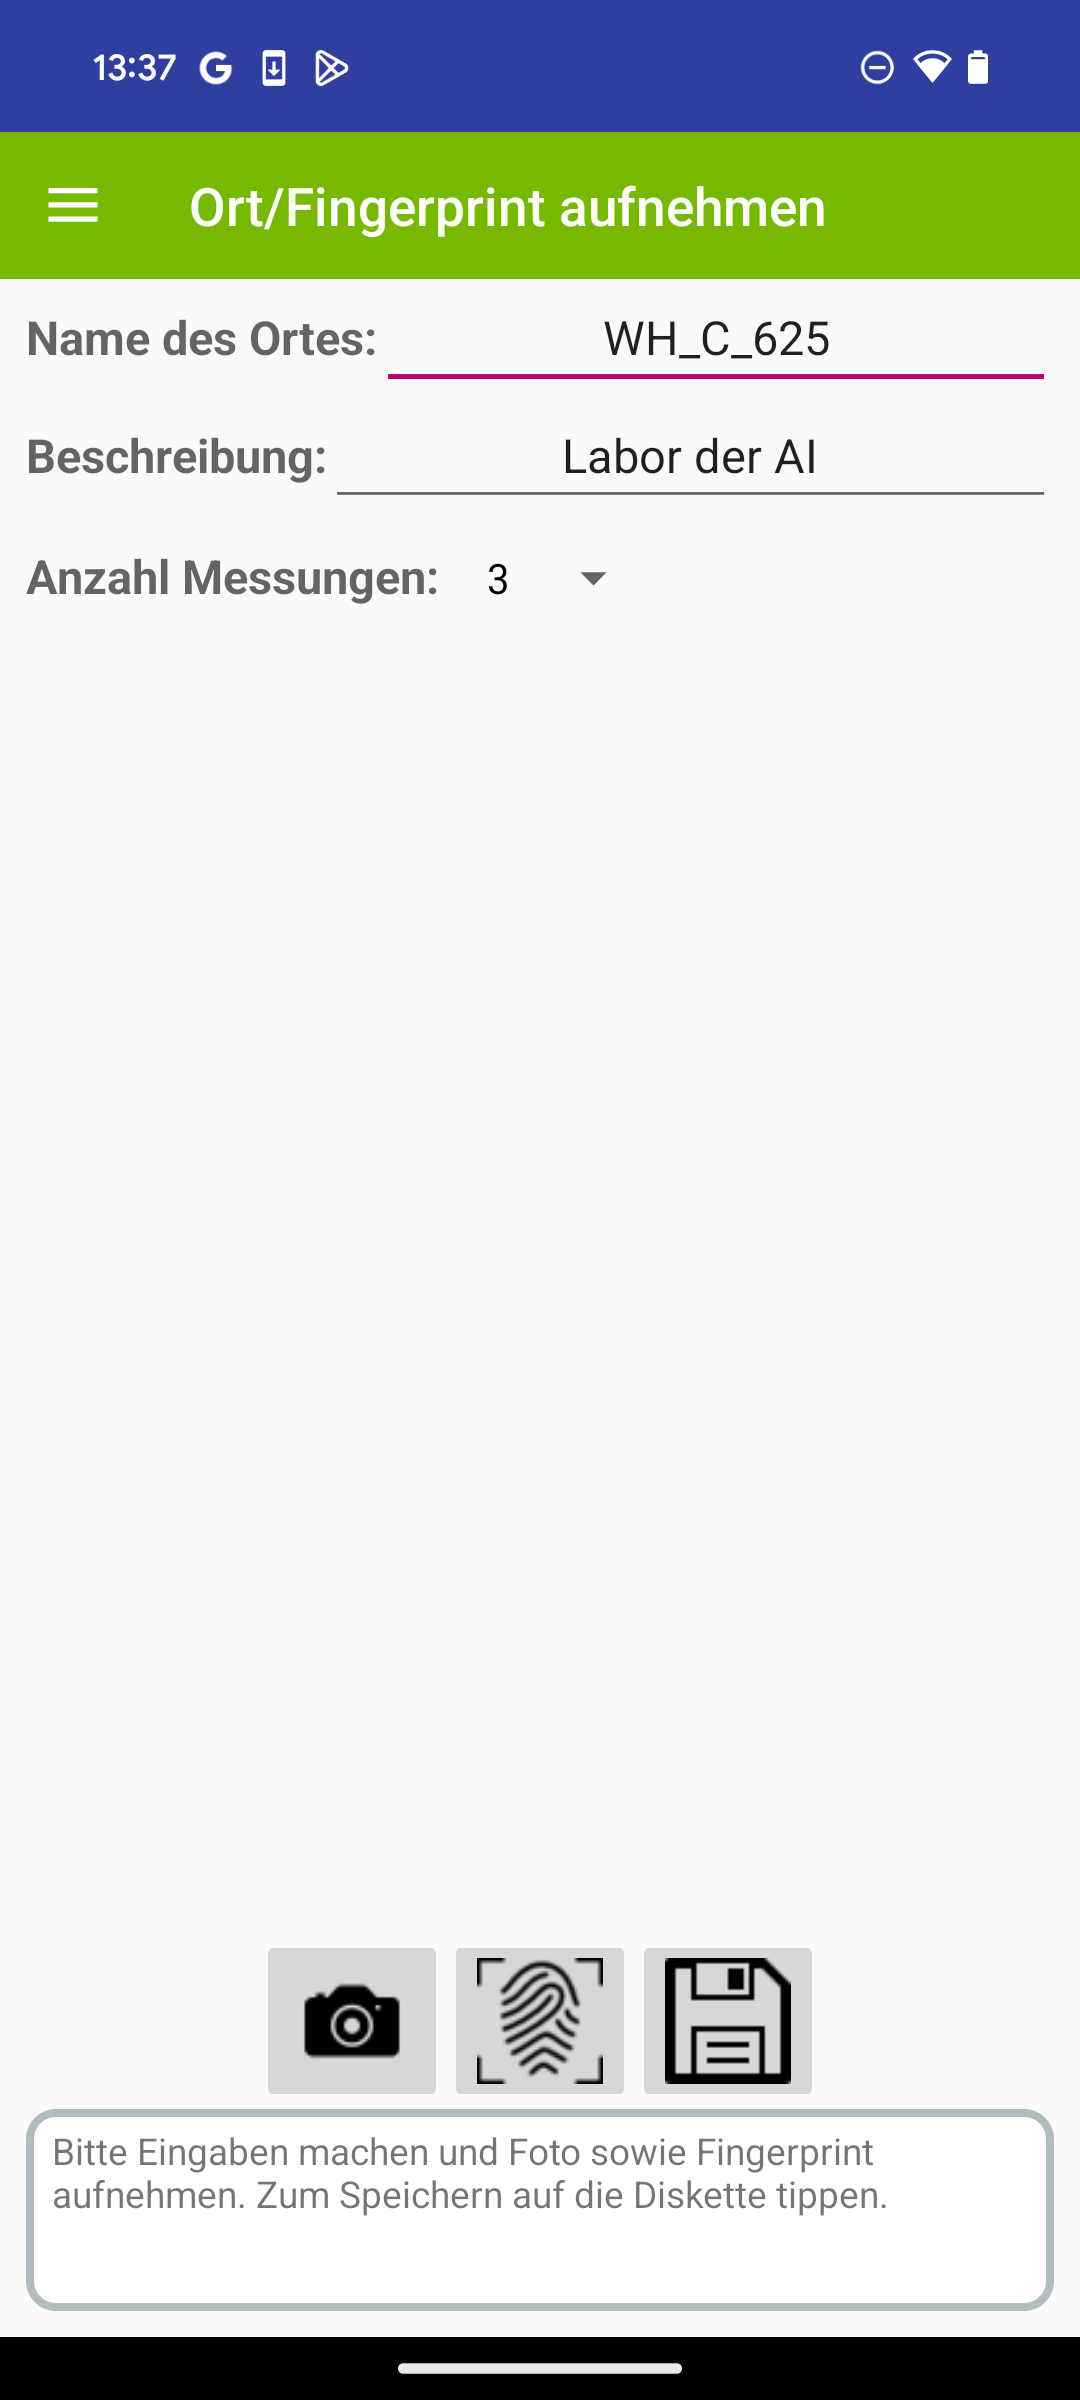
\includegraphics[width=0.3\textwidth]{images/screenshots/capture.png}
    \caption{Menüpunkt \textit{Ort/Fingerprint aufnehmen} der \textit{BVG Detection}-App}
    \label{fig:bvg_detection_capture}
\end{figure}

Unter dem Menüpunkt \textit{Fingerprints verwalten} (siehe Abbildung \ref{fig:bild1}) können alle Räume inklusive Messungen der Messungen (siehe Abbildung \ref{fig:bild2}) und den darin enthaltenen Access Points (siehe Abbildung \ref{fig:fingerprints-verwalten}) angezeigt werden.

\begin{figure}[h!]
    \centering
    \begin{subfigure}[b]{0.3\textwidth}
        \centering
        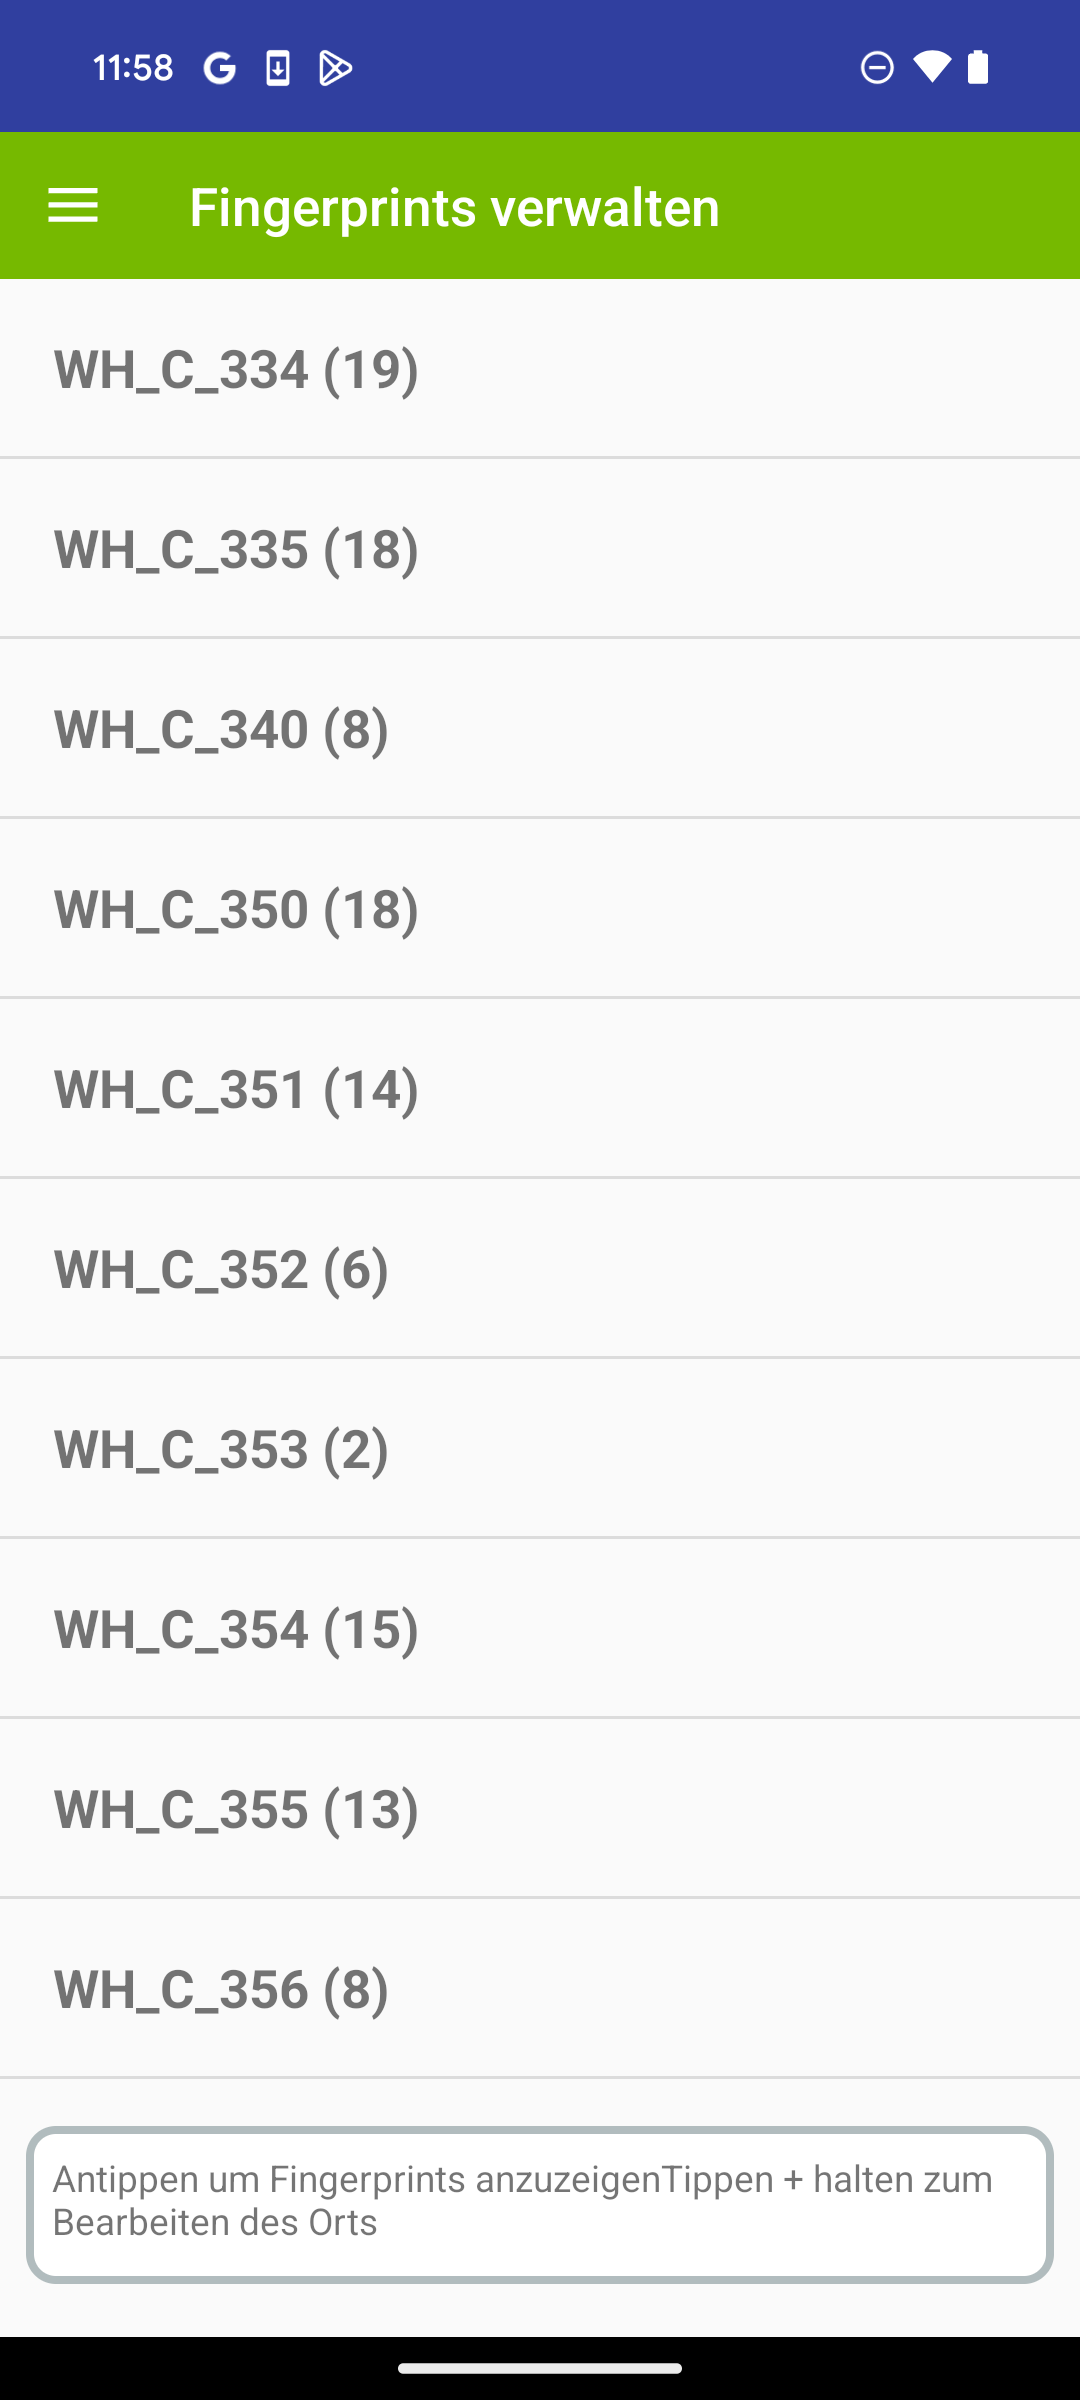
\includegraphics[width=\textwidth]{images/screenshots/all_rooms.png}
        \caption{Übersicht der gespeicherten Orte}
        \label{fig:bild1}
    \end{subfigure}
    \hfill
    \begin{subfigure}[b]{0.3\textwidth}
        \centering
        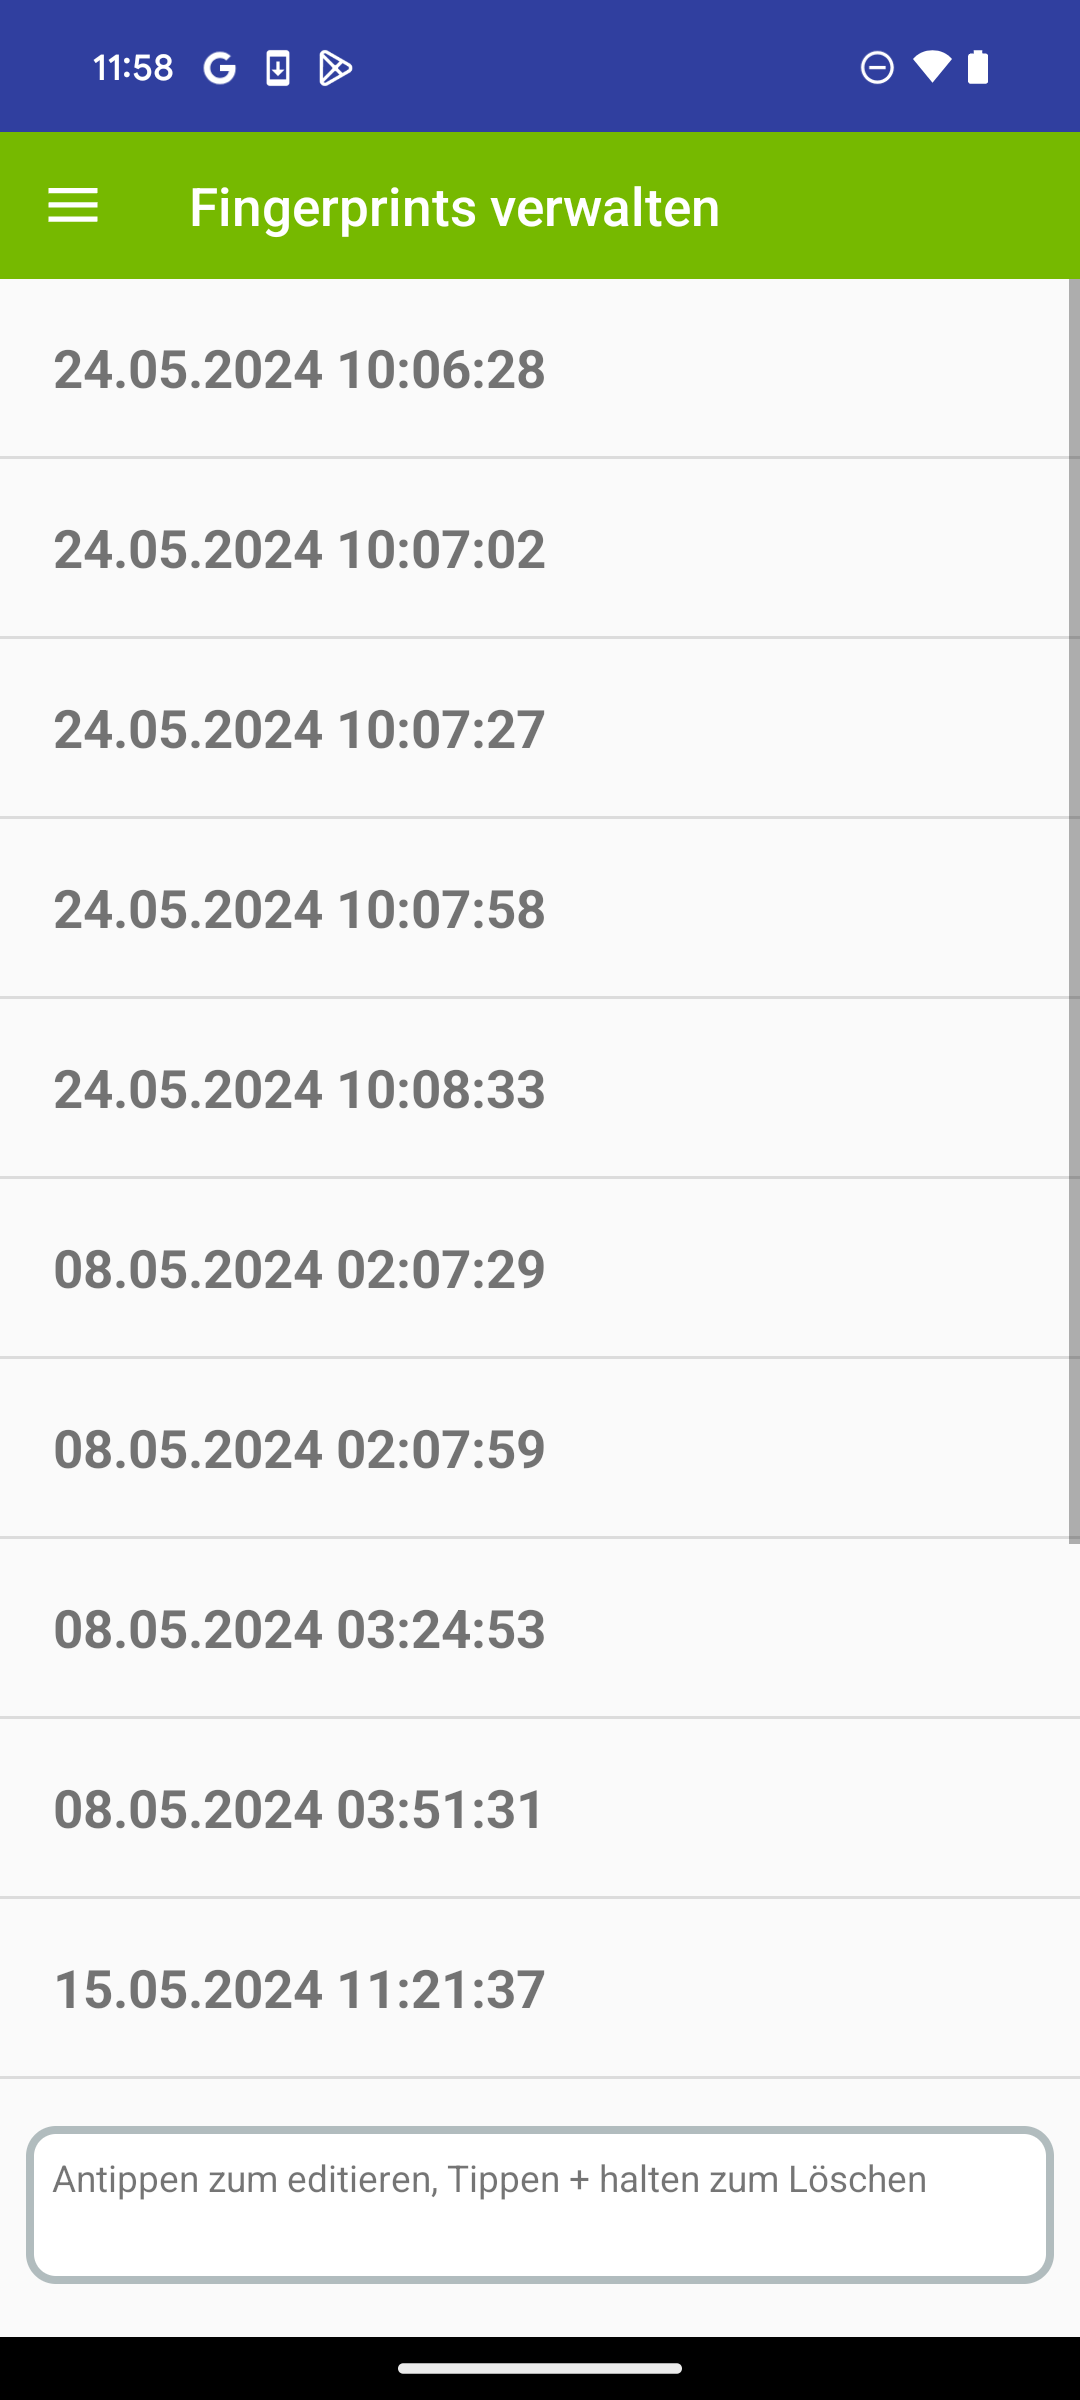
\includegraphics[width=\textwidth]{images/screenshots/all_measurements.png}
        \caption{Übersicht der Messungen eines Raumes}
        \label{fig:bild2}
    \end{subfigure}
    \hfill
    \begin{subfigure}[b]{0.3\textwidth}
        \centering
        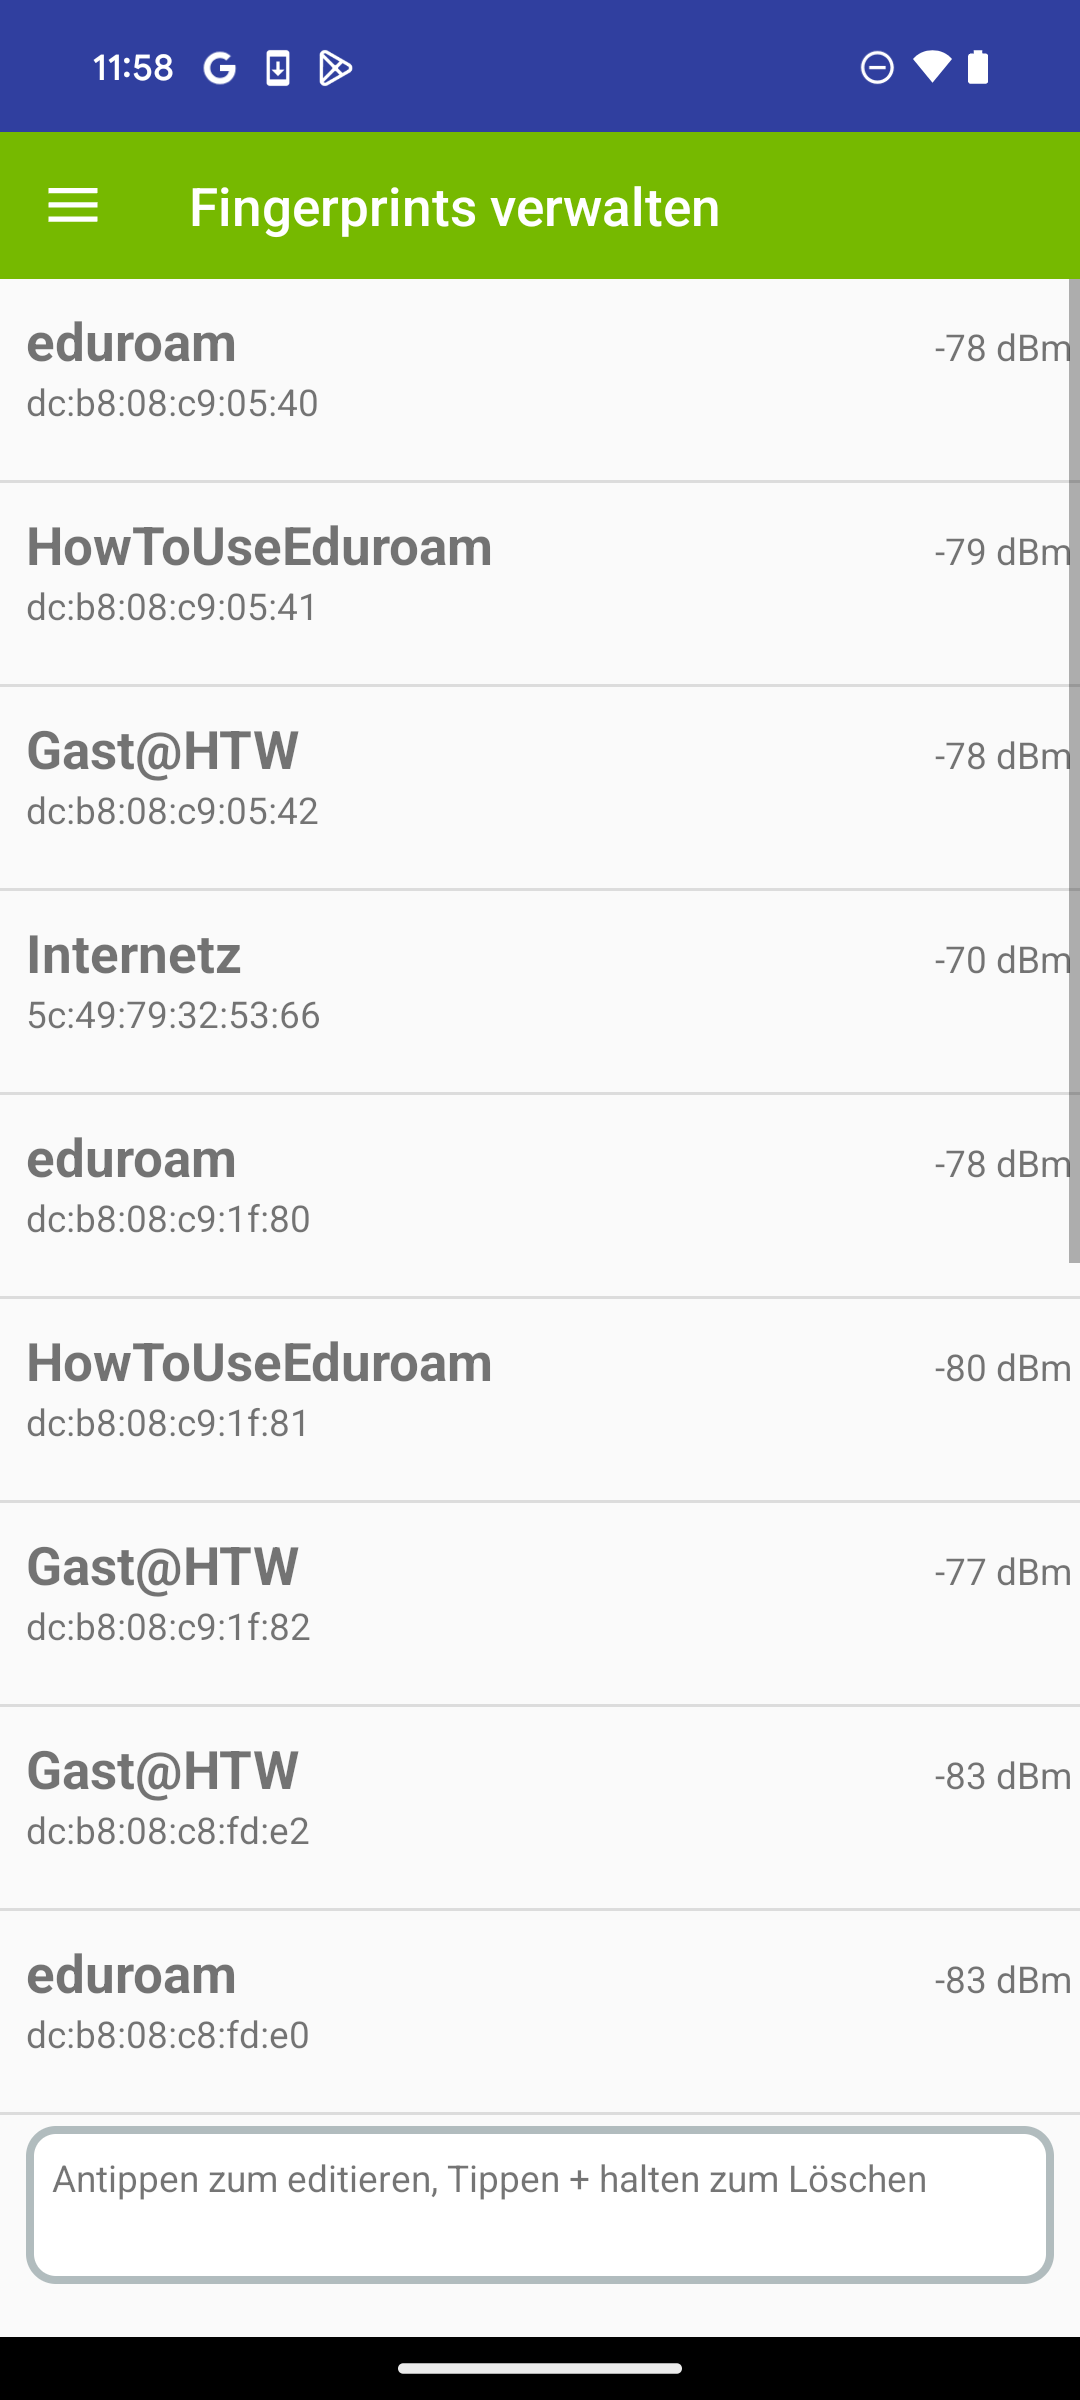
\includegraphics[width=\textwidth]{images/screenshots/fingerprint.png}
        \caption{Übersicht der Access Points einer Messung}
        \label{fig:bild3}
    \end{subfigure}
    \caption{Menüpunkt \textit{Fingerprints verwalten} der \textit{BVG Detection}-App}
    \label{fig:fingerprints-verwalten}
\end{figure}

Die kompilierte Version der App ist in dem \textit{GitLab}-Repository dieser Arbeit in dem Unterordner \texttt{bvg-detection-app} zu finden und in dem \textit{GitHub}-Repository der \textit{BVG Detection} App (\url{https://github.com/OpenHistoricalDataMap/BVGDetection}) auf dem Branch \texttt{v2}.

\subsection{Austausch der Daten}

Für den Austausch der Daten wurde der Menüpunkt \textit{Datenbank teilen} (siehe Abbildung \ref{fig:bvg_detection_share_database}) hinzugefügt. Unter diesem Menüpunkt können die gespeicherter Fingerprints per Bluetooth an andere Geräte gesendet werden bzw. von anderen Geräten empfangen werden und an die API aus Kapitel \ref{api} gesendet bzw. von dieser empfangen werden. 

Damit die Daten über Bluetooth ausgetauscht werden können, müssen beide Geräte eine Blue\-tooth-Verbindung eingehen. Dazu muss eins der beiden Geräte einen \texttt{BluetoothSocket} und das andere Gerät einen \texttt{BluetoothServerSocket} öffnen. Dies geschieht über die beiden Buttons \textit{Listen} und \textit{List Devices}. Im Anschluss werden alle sichtabren Geräte in einer Liste angezeigt und das entsprechende Gerät kann ausgewählt werden. Nachdem beide Geräte eine Bluetooth Verbindung aufgebaut haben, wird das in der App in dem Statustextfeld angezeit und über den Button \textit{Send} kann der Transfer der Daten gestartet werden.

Die zu übertragenden Messdaten werden aus der \textit{SQLite}-Datenbank des sendenden Geräts in einem \textit{JSON}-Array gesammelt. Anschließend wird dieses Array durchlaufen und jeder Eintrag in ein Byte-Array umgewandelt, welches dann über die Bluetooth Verbindung an den Empfänger gesendet werden kann.

Um die Struktur der gesendeten Daten zu kennzeichnen und die Nachrichten korrekt zu trennen, wird zwischen den einzelnen Messungen das Trennzeichen (\texttt{MESSAGE\_SPLIT \allowbreak = \allowbreak \grqq{}\_NEW\_MESSAGE\_\allowbreak \grqq{}}) eingefügt und am Ende der gesamten Übertragung wird das Endzeichen (\texttt{MESSAGE\_END \allowbreak = \allowbreak \grqq{}\_MESSAGE\_END\_\allowbreak \grqq{}}) gesendet. Dadurch wird der Empfänger darüber informiert, dass die Übertragung abgeschlossen ist. Der Empfänger sammelt die eingehenden Daten, bis das Endzeichen erkannt wird. Anschließend werden die gesammelten Daten wieder in ein \textit{JSON}-Array konvertiert und in der \textit{SQLite}-Datenbank des Empfängers gespeichert.

Für den Austausch der Daten mit der API aus Kapitel \ref{api} muss sich das Smartphone in dem Netzwerk der HTW Berlin befinden. Wenn das der Fall ist kann über den Button \textit{Send to API} die Übertragung der Messungen an die API gestartet werden. Über den Button \textit{Receive from API} werden alle Fingerprints die in der \textit{MariaDB} auf dem Server gespeichert sind empfangen und lokal gespeichert werden 

\begin{figure}[h]
    \centering
    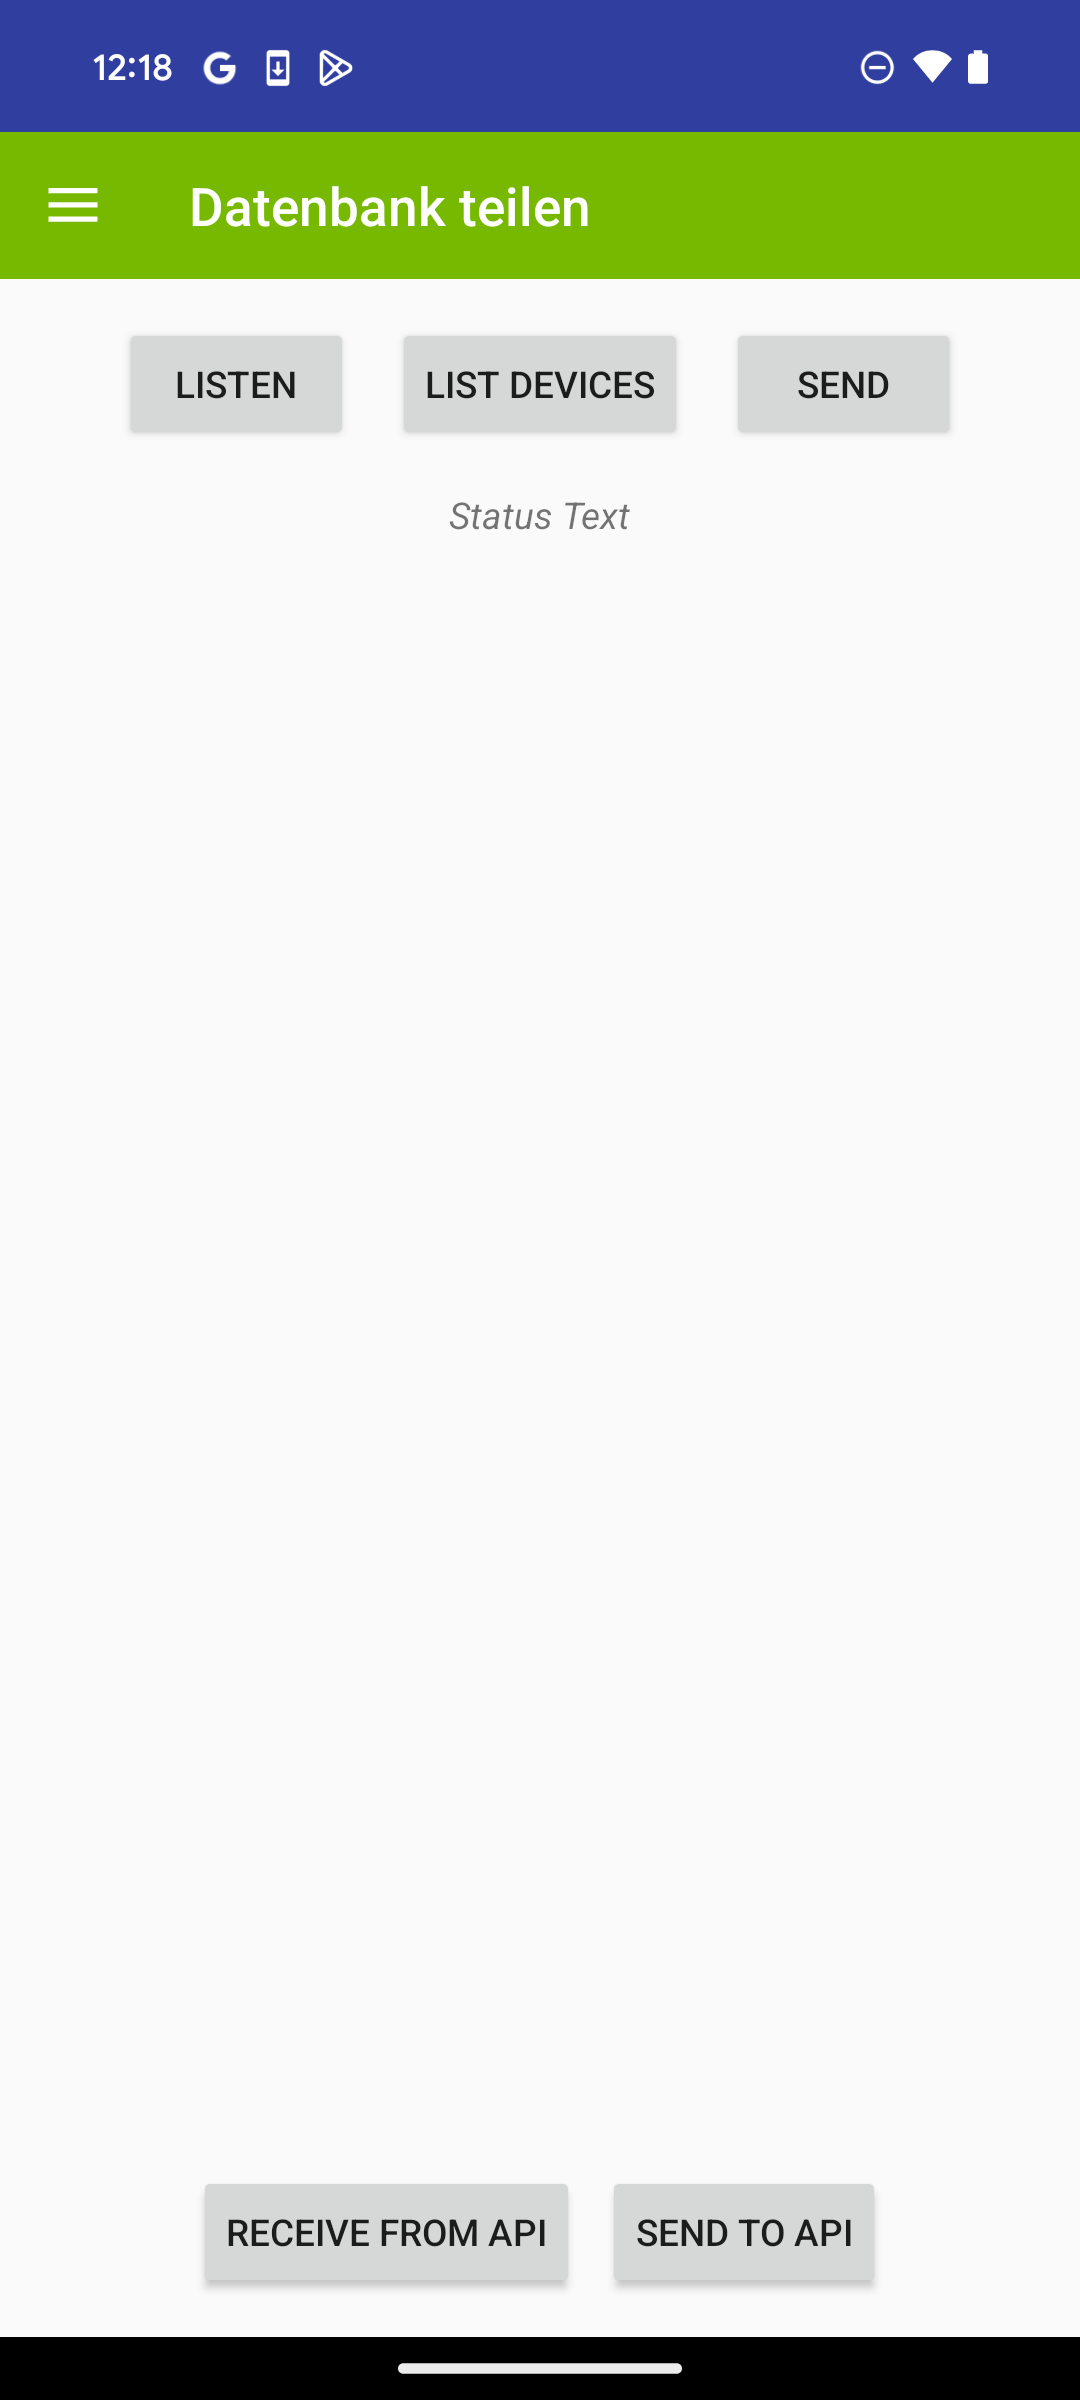
\includegraphics[width=0.3\textwidth]{images/screenshots/share_database.png}
    \caption{Menüpunkt \textit{Datenbank teilen} der \textit{BVG Detection}-App}
    \label{fig:bvg_detection_share_database}
\end{figure}

Da die API auf einem HTTP-Server läuft und kein SSL Zertifikat hat, muss der Zugriff explizit erlaubt werden, indem die IP-Adresse des Servers in der Netzwerkkonfiguration der App eingetragen wird. Sollte sich die IP-Adresse des Servers ändern, muss diese manuell im Quellcode der App geändert werden.

\begin{lstlisting}[caption={Netzwerkkonfiguration der App}]
<?xml version="1.0" encoding="utf-8"?>
<network-security-config>
    <domain-config cleartextTrafficPermitted="true">
    <domain includeSubdomains="true">141.45.212.246</domain>
    </domain-config>
</network-security-config>    
\end{lstlisting}

\subsection{Ortung von Räumen}

Die Ortung kann über den Menüpunkt \textit{Standort ermitteln} (siehe Abbildung \ref{fig:app-localize-1}) gestartet werden und wird lokal auf dem Gerät ausgeführt. Dazu wurden die in dieser Arbeit untersuchten Algorithmen (\gls{knn}, \gls{svm} und Random Forest), die dazugehörigen Parameter und die Datenaufbereitungsschritte (siehe Kapitel \ref{datenaufbereitung}) implementiert. Aus dem Grund, dass für die Algorithmen in der API die Python Bibliothek \textit{scikit-learn} verwendet wurde und diese nicht unter Android verwendet werden kann, wurden die Algorithmen in Java nachimplementiert. 

Der \gls{knn} und Random Forest Algorithmus wurden nach den Vorlagen von \textit{Kenzo Takahashi} und \textit{Florian Zyprian}, in welchen die Algorithmen von \textit{scikit-learn} nachimplementiert wurden, implementiert\mycitefoot{kenzotakahashiKNearestNeighbor}\textsuperscript{,}\mycitefoot{konfuzioRandomForest}. Für die Implementierung des \gls{svm} Algorithmus wurde die Bibliothek \textit{AndroidLibSvm} (\url{https://github.com/yctung/AndroidLibSVM}), welche eine Open-Source Implementierung der \textit{LIBSVM} Bibliothek (\url{https://www.csie.ntu.edu.tw/~cjlin/libsvm/}) ist, verwendet.

Die Algorithmen inklusive Parameter und die verschiedenen Methoden zur Aufbereitung der Daten können in den Einstellungen (siehe Abbildungen \ref{fig:app-localize-2} und \ref{fig:app-localize-3}) ausgewählt werden und werden bei der Ortung (siehe Abbildung \ref{fig:app-localize-1}) angezeigt.

\begin{figure}[h!]
    \centering
    \begin{subfigure}[b]{0.3\textwidth}
        \centering
        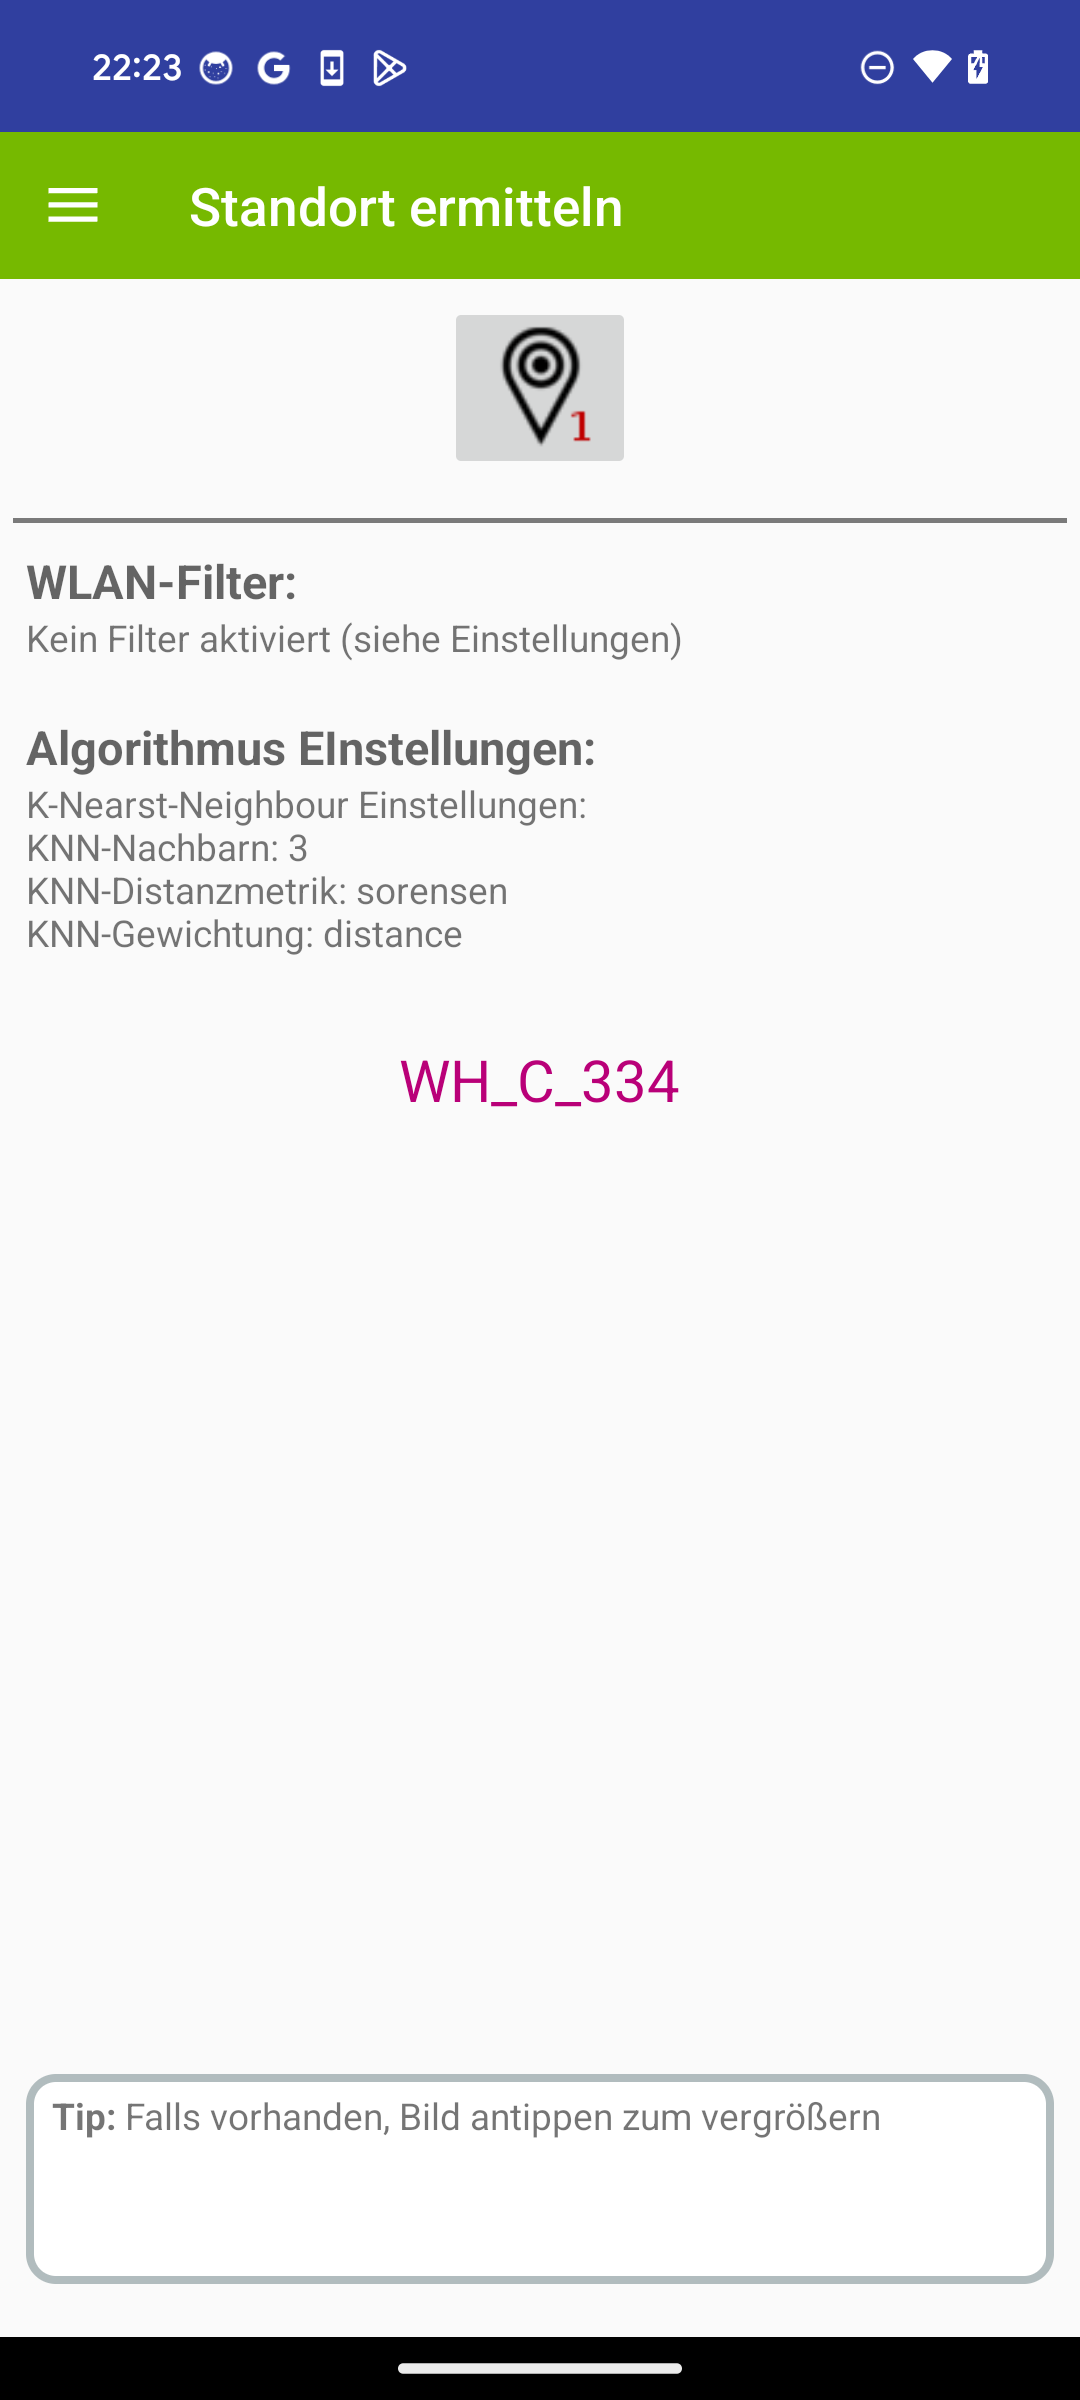
\includegraphics[width=\textwidth]{images/screenshots/localize.png}
        \caption{Menüpunkt \textit{Standort ermitteln}}
        \label{fig:app-localize-1}
    \end{subfigure}
    \hfill
    \begin{subfigure}[b]{0.3\textwidth}
        \centering
        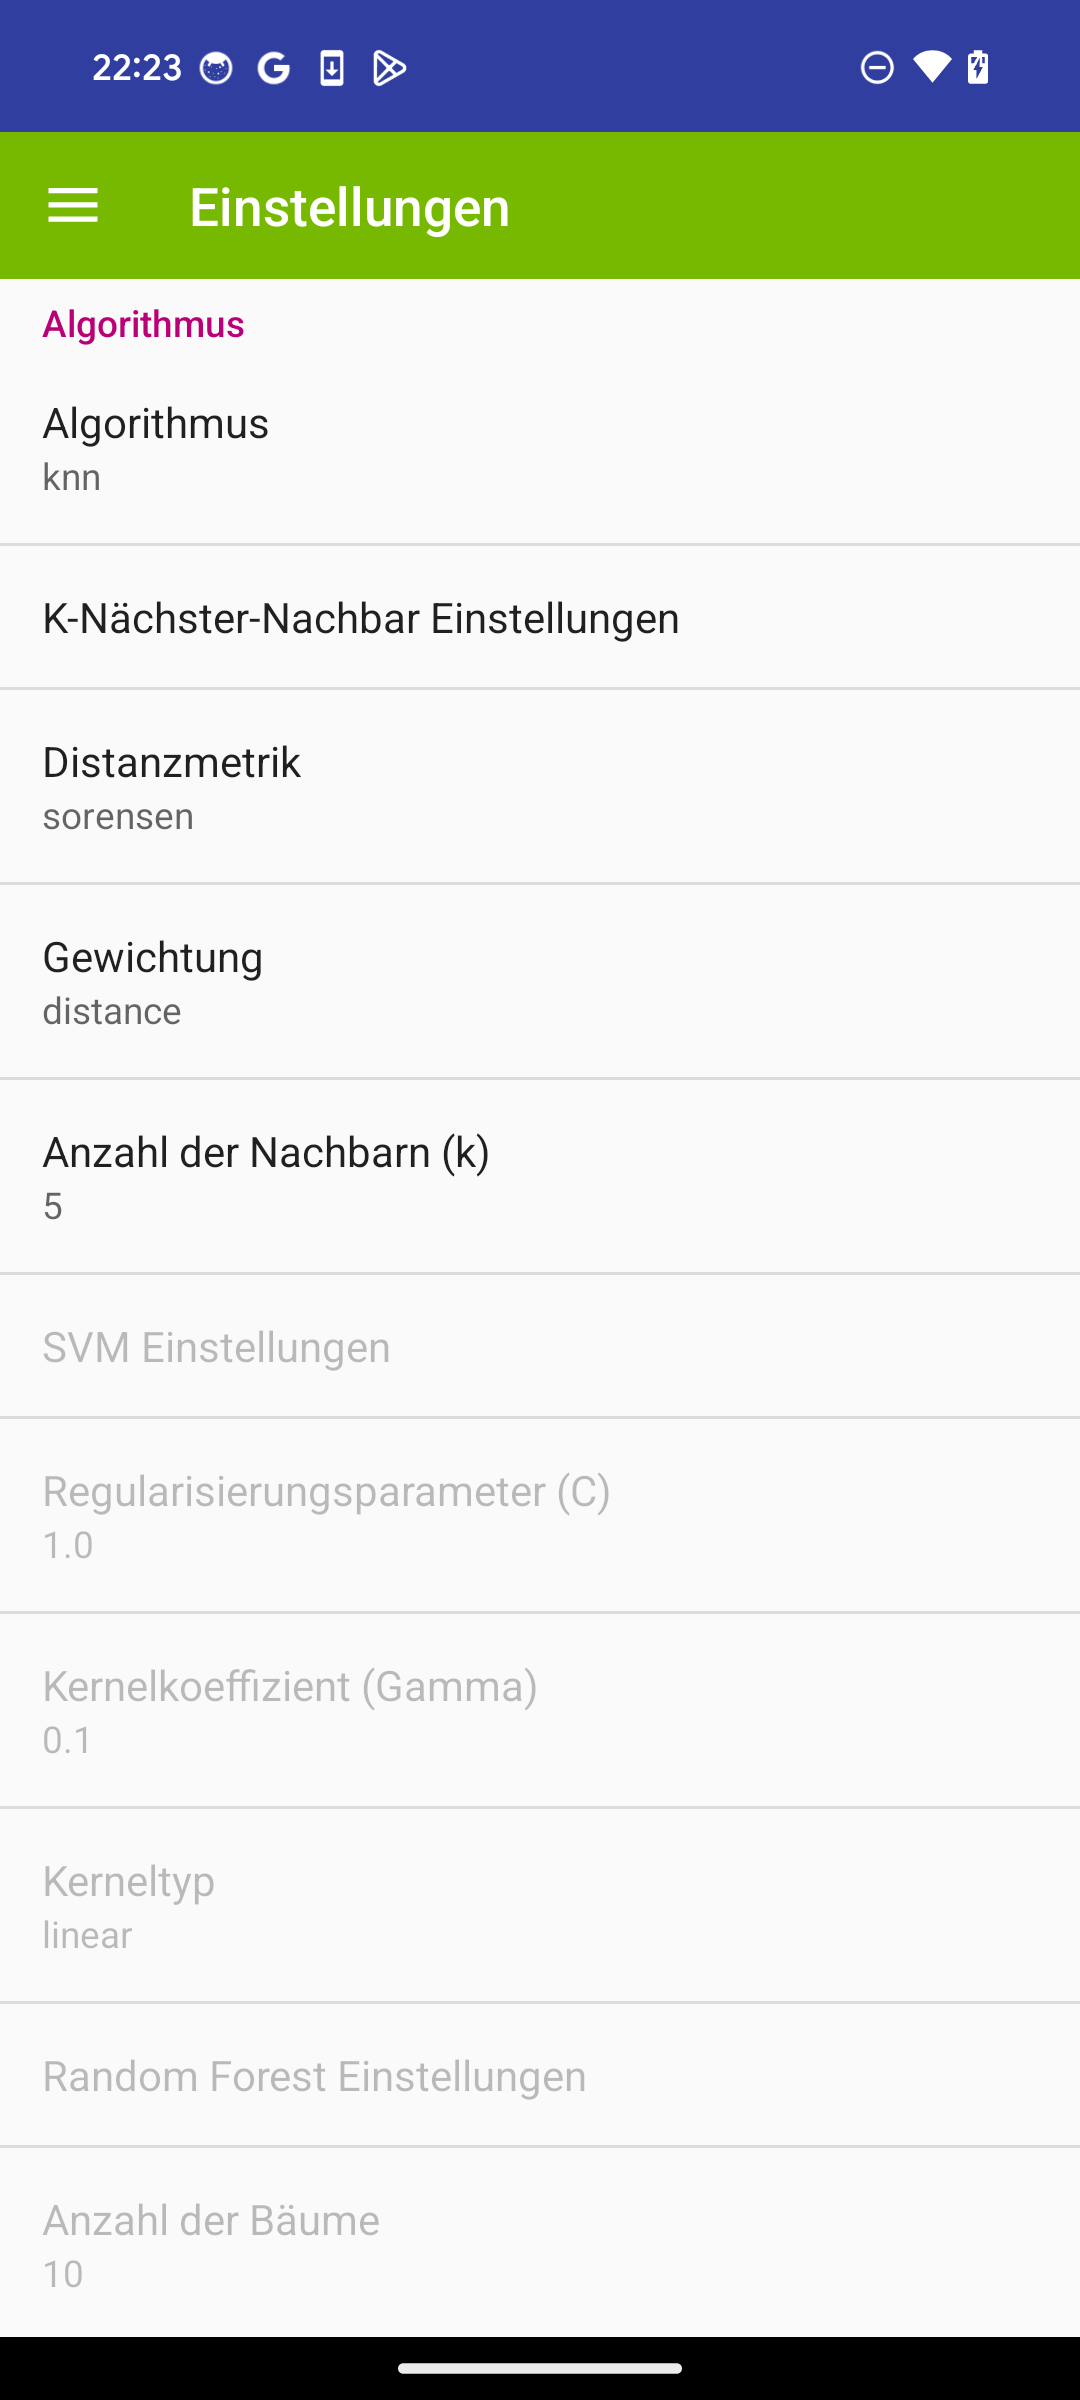
\includegraphics[width=\textwidth]{images/screenshots/settings_1.png}
        \caption{Einstellungen der Algorithmen und deren Parameter}
        \label{fig:app-localize-2}
    \end{subfigure}
    \hfill
    \begin{subfigure}[b]{0.3\textwidth}
        \centering
        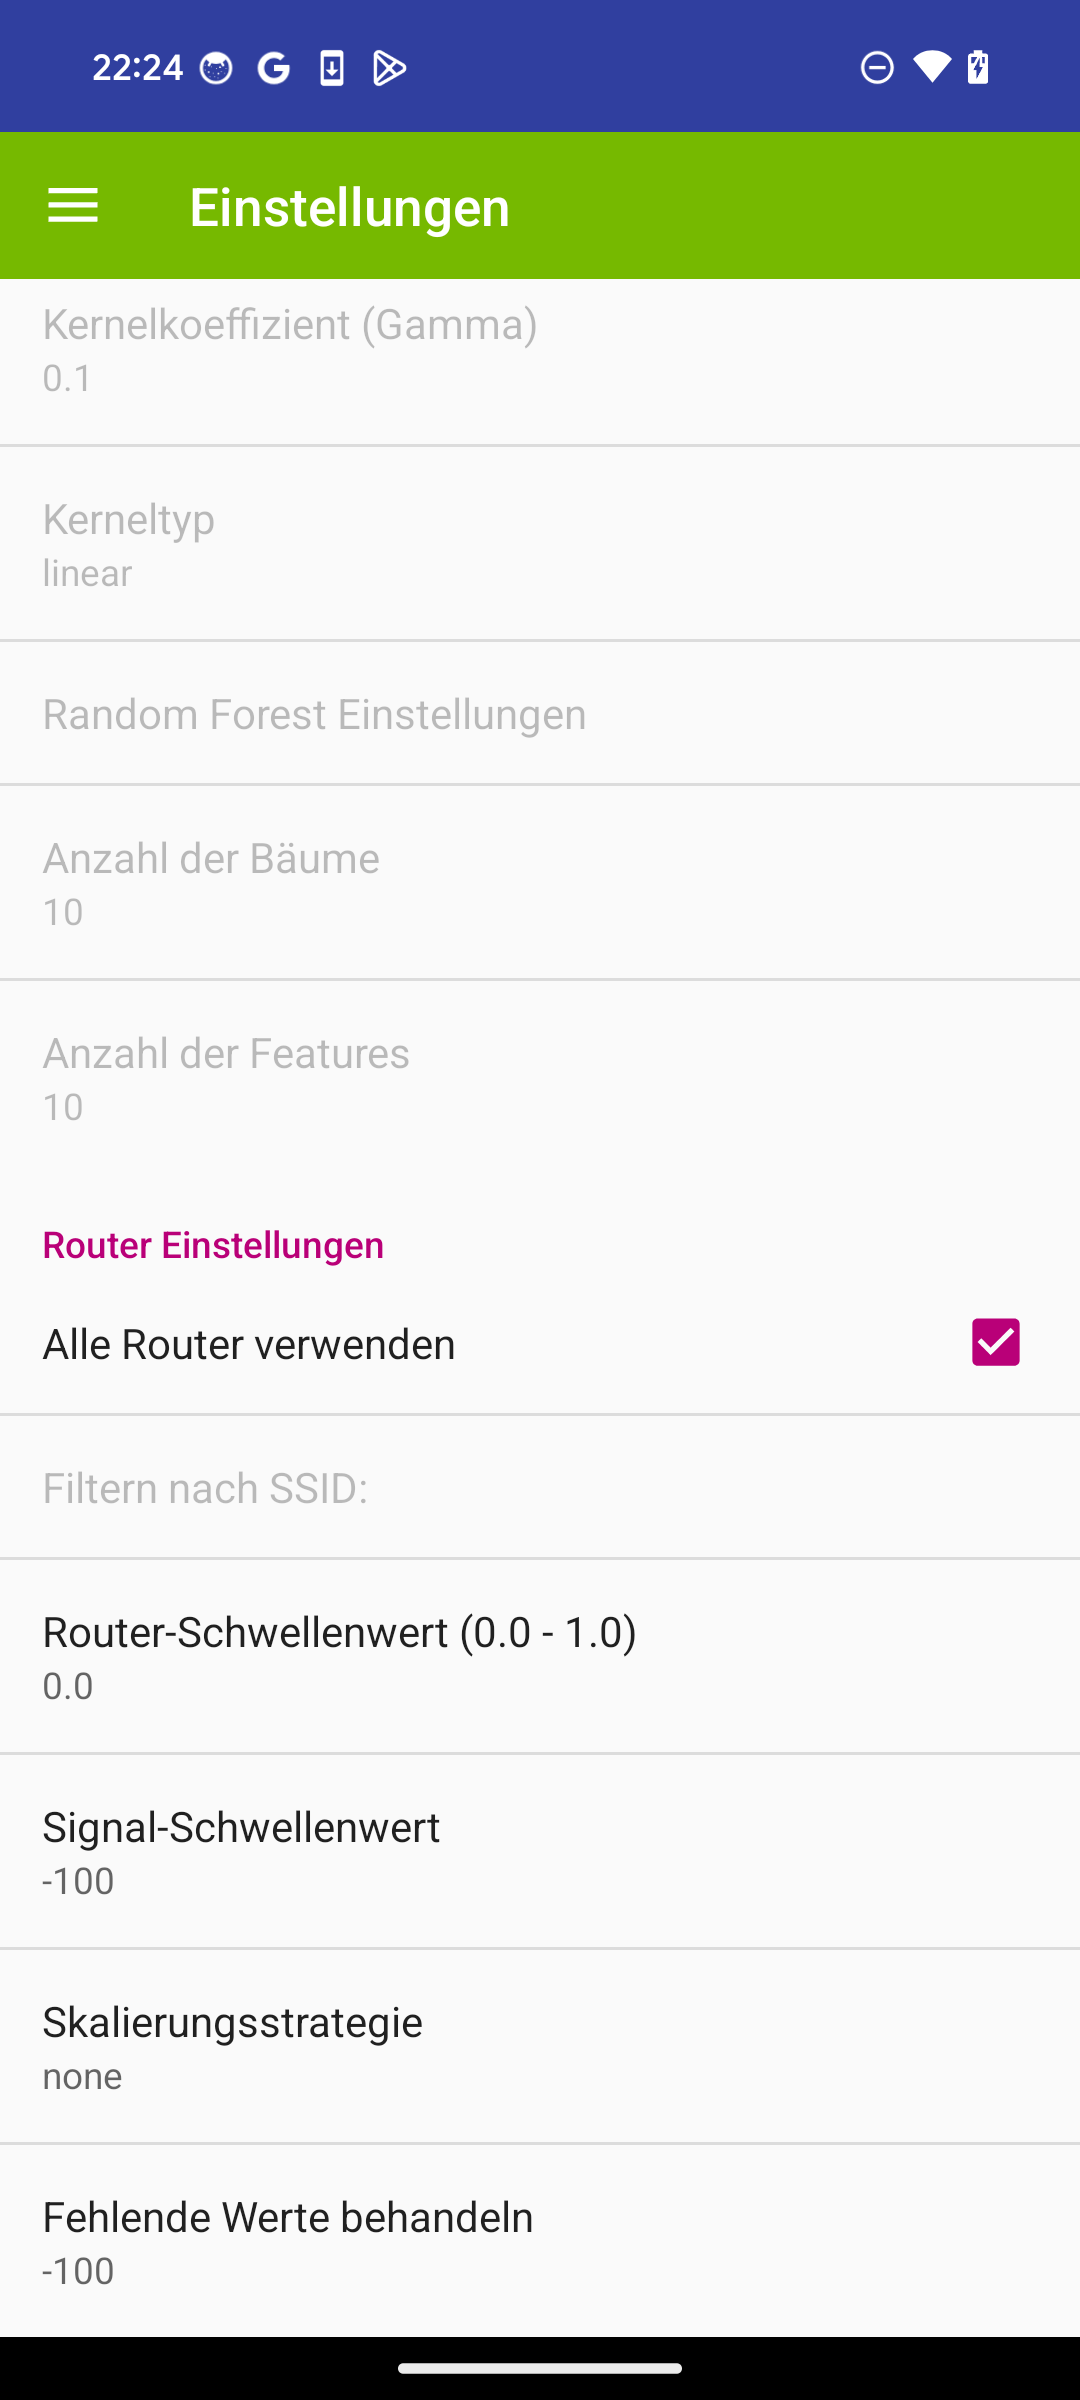
\includegraphics[width=\textwidth]{images/screenshots/settings_2.png}
        \caption{Übersicht der Access Points einer Messung}
        \label{fig:app-localize-3}
    \end{subfigure}
    \caption{Einstellungen der Datenaufbereitungsmethoden}
    \label{fig:app-localize-4}
\end{figure}

\section{Quellcode der Microcontroller}

Damit Microcontroller wie zum Beispiel der \textit{ESP32} seine Position bestimmen kann, muss dieser einen WiFi-Scan durchführen und die Daten an die API aus Kapitel \ref{api} senden. Dafür wurde ein \textit{MicroPython}-Script geschrieben, dass in dem Code Beispiel \ref{lst:esp32} dargestellt ist.

\begin{lstlisting}[caption={\textit{MicroPython}-Quellcode für die Durchführung eines WiFi-Scans und die Raumbestimmung über die API}, label={lst:esp32}]
import network
import urequests
import utime

# Initialize the Wi-Fi interface globally
wlan = network.WLAN(network.STA_IF)

# Function to connect to a Wi-Fi network
def connect_to_wifi(ssid, password):
    global wlan
    wlan.active(True)
    
    if not wlan.isconnected():
        print(f"Connecting to {ssid}...")
        wlan.connect(ssid, password)
        
        while not wlan.isconnected():
            print("Attempting to establish connection...")
            utime.sleep(1)
    
    print("Connected to Wi-Fi!")

# Function to scan available Wi-Fi networks and send the data to an API
def scan_and_send(api_route):
    global wlan
    
    # Scan for available networks
    networks = wlan.scan()
    
    # Prepare the data structure for the API
    routers = []
    for network in networks:
        bssid = ":".join("{:02x}".format(byte) for byte in network[1])
        signal_strength = network[3]
        ssid = network[0].decode('utf-8')
        
        if len(ssid) > 0:
            routers.append({
                "ssid": ssid,
                "bssid": bssid,
                "signal_strength": signal_strength
            })
    
    data = {
        "routers": routers
    }
    
    # Send the data via a POST request to the API
    try:
        response = urequests.post(api_route, json=data)
        if response.status_code == 200:
            response_json = response.json()
            print(f"Room Prediction: {response_json['room_name']}")
        else:
            print(f"Error in room prediction: {response.status_code} - {response.text}")
    except Exception as e:
        print(f"Error sending data: {e}")

# Main function
def main(ssid, password, api_route):
    connect_to_wifi(ssid, password)
    
    # Perform the Wi-Fi scan and send the data to the API
    scan_and_send(api_route)

if __name__ == '__main__':
    # Define SSID, password, and API route here
    ssid = 'Rechnernetze'
    password = ''
    api_route = 'http://141.45.212.246:8000/measurements/predict'
    
    main(ssid, password, api_route)
\end{lstlisting}    
